% Options for packages loaded elsewhere
\PassOptionsToPackage{unicode}{hyperref}
\PassOptionsToPackage{hyphens}{url}
%
\documentclass[
]{book}
\usepackage{amsmath,amssymb}
\usepackage{lmodern}
\usepackage{ifxetex,ifluatex}
\ifnum 0\ifxetex 1\fi\ifluatex 1\fi=0 % if pdftex
  \usepackage[T1]{fontenc}
  \usepackage[utf8]{inputenc}
  \usepackage{textcomp} % provide euro and other symbols
\else % if luatex or xetex
  \usepackage{unicode-math}
  \defaultfontfeatures{Scale=MatchLowercase}
  \defaultfontfeatures[\rmfamily]{Ligatures=TeX,Scale=1}
\fi
% Use upquote if available, for straight quotes in verbatim environments
\IfFileExists{upquote.sty}{\usepackage{upquote}}{}
\IfFileExists{microtype.sty}{% use microtype if available
  \usepackage[]{microtype}
  \UseMicrotypeSet[protrusion]{basicmath} % disable protrusion for tt fonts
}{}
\makeatletter
\@ifundefined{KOMAClassName}{% if non-KOMA class
  \IfFileExists{parskip.sty}{%
    \usepackage{parskip}
  }{% else
    \setlength{\parindent}{0pt}
    \setlength{\parskip}{6pt plus 2pt minus 1pt}}
}{% if KOMA class
  \KOMAoptions{parskip=half}}
\makeatother
\usepackage{xcolor}
\IfFileExists{xurl.sty}{\usepackage{xurl}}{} % add URL line breaks if available
\IfFileExists{bookmark.sty}{\usepackage{bookmark}}{\usepackage{hyperref}}
\hypersetup{
  pdftitle={Modelos lineales generalizados con R},
  pdfauthor={Jaime Isaac y Gerson Rivera},
  hidelinks,
  pdfcreator={LaTeX via pandoc}}
\urlstyle{same} % disable monospaced font for URLs
\usepackage{color}
\usepackage{fancyvrb}
\newcommand{\VerbBar}{|}
\newcommand{\VERB}{\Verb[commandchars=\\\{\}]}
\DefineVerbatimEnvironment{Highlighting}{Verbatim}{commandchars=\\\{\}}
% Add ',fontsize=\small' for more characters per line
\usepackage{framed}
\definecolor{shadecolor}{RGB}{248,248,248}
\newenvironment{Shaded}{\begin{snugshade}}{\end{snugshade}}
\newcommand{\AlertTok}[1]{\textcolor[rgb]{0.94,0.16,0.16}{#1}}
\newcommand{\AnnotationTok}[1]{\textcolor[rgb]{0.56,0.35,0.01}{\textbf{\textit{#1}}}}
\newcommand{\AttributeTok}[1]{\textcolor[rgb]{0.77,0.63,0.00}{#1}}
\newcommand{\BaseNTok}[1]{\textcolor[rgb]{0.00,0.00,0.81}{#1}}
\newcommand{\BuiltInTok}[1]{#1}
\newcommand{\CharTok}[1]{\textcolor[rgb]{0.31,0.60,0.02}{#1}}
\newcommand{\CommentTok}[1]{\textcolor[rgb]{0.56,0.35,0.01}{\textit{#1}}}
\newcommand{\CommentVarTok}[1]{\textcolor[rgb]{0.56,0.35,0.01}{\textbf{\textit{#1}}}}
\newcommand{\ConstantTok}[1]{\textcolor[rgb]{0.00,0.00,0.00}{#1}}
\newcommand{\ControlFlowTok}[1]{\textcolor[rgb]{0.13,0.29,0.53}{\textbf{#1}}}
\newcommand{\DataTypeTok}[1]{\textcolor[rgb]{0.13,0.29,0.53}{#1}}
\newcommand{\DecValTok}[1]{\textcolor[rgb]{0.00,0.00,0.81}{#1}}
\newcommand{\DocumentationTok}[1]{\textcolor[rgb]{0.56,0.35,0.01}{\textbf{\textit{#1}}}}
\newcommand{\ErrorTok}[1]{\textcolor[rgb]{0.64,0.00,0.00}{\textbf{#1}}}
\newcommand{\ExtensionTok}[1]{#1}
\newcommand{\FloatTok}[1]{\textcolor[rgb]{0.00,0.00,0.81}{#1}}
\newcommand{\FunctionTok}[1]{\textcolor[rgb]{0.00,0.00,0.00}{#1}}
\newcommand{\ImportTok}[1]{#1}
\newcommand{\InformationTok}[1]{\textcolor[rgb]{0.56,0.35,0.01}{\textbf{\textit{#1}}}}
\newcommand{\KeywordTok}[1]{\textcolor[rgb]{0.13,0.29,0.53}{\textbf{#1}}}
\newcommand{\NormalTok}[1]{#1}
\newcommand{\OperatorTok}[1]{\textcolor[rgb]{0.81,0.36,0.00}{\textbf{#1}}}
\newcommand{\OtherTok}[1]{\textcolor[rgb]{0.56,0.35,0.01}{#1}}
\newcommand{\PreprocessorTok}[1]{\textcolor[rgb]{0.56,0.35,0.01}{\textit{#1}}}
\newcommand{\RegionMarkerTok}[1]{#1}
\newcommand{\SpecialCharTok}[1]{\textcolor[rgb]{0.00,0.00,0.00}{#1}}
\newcommand{\SpecialStringTok}[1]{\textcolor[rgb]{0.31,0.60,0.02}{#1}}
\newcommand{\StringTok}[1]{\textcolor[rgb]{0.31,0.60,0.02}{#1}}
\newcommand{\VariableTok}[1]{\textcolor[rgb]{0.00,0.00,0.00}{#1}}
\newcommand{\VerbatimStringTok}[1]{\textcolor[rgb]{0.31,0.60,0.02}{#1}}
\newcommand{\WarningTok}[1]{\textcolor[rgb]{0.56,0.35,0.01}{\textbf{\textit{#1}}}}
\usepackage{longtable,booktabs,array}
\usepackage{calc} % for calculating minipage widths
% Correct order of tables after \paragraph or \subparagraph
\usepackage{etoolbox}
\makeatletter
\patchcmd\longtable{\par}{\if@noskipsec\mbox{}\fi\par}{}{}
\makeatother
% Allow footnotes in longtable head/foot
\IfFileExists{footnotehyper.sty}{\usepackage{footnotehyper}}{\usepackage{footnote}}
\makesavenoteenv{longtable}
\usepackage{graphicx}
\makeatletter
\def\maxwidth{\ifdim\Gin@nat@width>\linewidth\linewidth\else\Gin@nat@width\fi}
\def\maxheight{\ifdim\Gin@nat@height>\textheight\textheight\else\Gin@nat@height\fi}
\makeatother
% Scale images if necessary, so that they will not overflow the page
% margins by default, and it is still possible to overwrite the defaults
% using explicit options in \includegraphics[width, height, ...]{}
\setkeys{Gin}{width=\maxwidth,height=\maxheight,keepaspectratio}
% Set default figure placement to htbp
\makeatletter
\def\fps@figure{htbp}
\makeatother
\setlength{\emergencystretch}{3em} % prevent overfull lines
\providecommand{\tightlist}{%
  \setlength{\itemsep}{0pt}\setlength{\parskip}{0pt}}
\setcounter{secnumdepth}{5}
\usepackage{booktabs}
\ifluatex
  \usepackage{selnolig}  % disable illegal ligatures
\fi
\usepackage[]{natbib}
\bibliographystyle{apalike}

\title{Modelos lineales generalizados con R}
\author{Jaime Isaac y Gerson Rivera}
\date{2021-04-28}

\begin{document}
\maketitle

{
\setcounter{tocdepth}{1}
\tableofcontents
}
\hypertarget{prerequisites}{%
\chapter{Prerequisites}\label{prerequisites}}

This is a \emph{sample} book written in \textbf{Markdown}. You can use anything that Pandoc's Markdown supports, e.g., a math equation \(a^2 + b^2 = c^2\).

The \textbf{bookdown} package can be installed from CRAN or Github:

\begin{Shaded}
\begin{Highlighting}[]
\FunctionTok{install.packages}\NormalTok{(}\StringTok{"bookdown"}\NormalTok{)}
\CommentTok{\# or the development version}
\CommentTok{\# devtools::install\_github("rstudio/bookdown")}
\end{Highlighting}
\end{Shaded}

Remember each Rmd file contains one and only one chapter, and a chapter is defined by the first-level heading \texttt{\#}.

To compile this example to PDF, you need XeLaTeX. You are recommended to install TinyTeX (which includes XeLaTeX): \url{https://yihui.org/tinytex/}.

\hypertarget{intro}{%
\chapter{Introduction}\label{intro}}

You can label chapter and section titles using \texttt{\{\#label\}} after them, e.g., we can reference Chapter \ref{intro}. If you do not manually label them, there will be automatic labels anyway, e.g., Chapter \ref{methods}.

Figures and tables with captions will be placed in \texttt{figure} and \texttt{table} environments, respectively.

\begin{Shaded}
\begin{Highlighting}[]
\FunctionTok{par}\NormalTok{(}\AttributeTok{mar =} \FunctionTok{c}\NormalTok{(}\DecValTok{4}\NormalTok{, }\DecValTok{4}\NormalTok{, .}\DecValTok{1}\NormalTok{, .}\DecValTok{1}\NormalTok{))}
\FunctionTok{plot}\NormalTok{(pressure, }\AttributeTok{type =} \StringTok{\textquotesingle{}b\textquotesingle{}}\NormalTok{, }\AttributeTok{pch =} \DecValTok{19}\NormalTok{)}
\end{Highlighting}
\end{Shaded}

\begin{figure}

{\centering 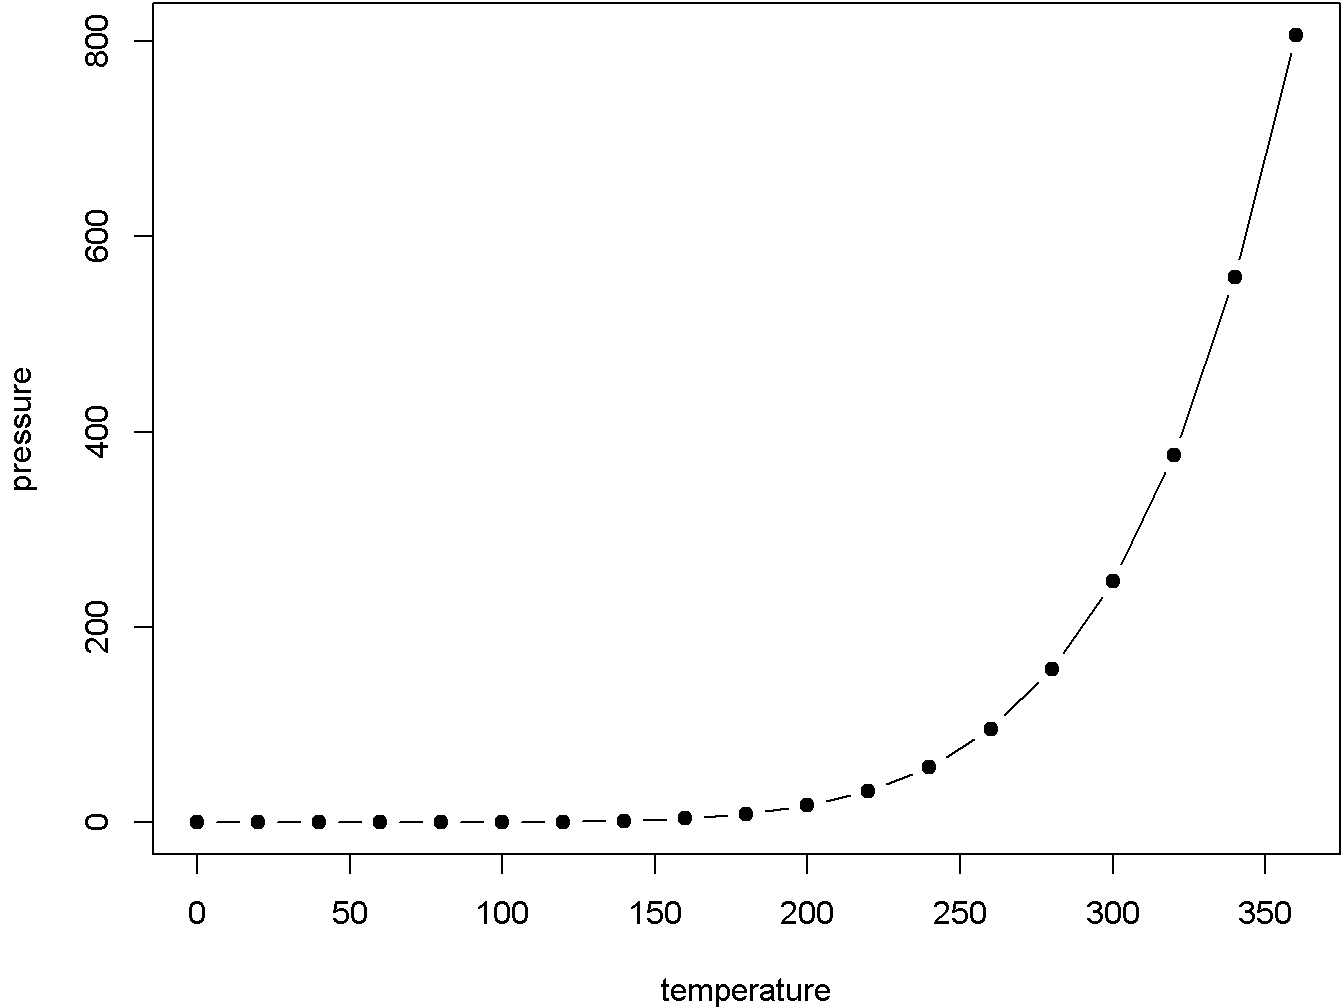
\includegraphics[width=0.8\linewidth]{bookglm_files/figure-latex/nice-fig-1} 

}

\caption{Here is a nice figure!}\label{fig:nice-fig}
\end{figure}

Reference a figure by its code chunk label with the \texttt{fig:} prefix, e.g., see Figure \ref{fig:nice-fig}. Similarly, you can reference tables generated from \texttt{knitr::kable()}, e.g., see Table \ref{tab:nice-tab}.

\begin{Shaded}
\begin{Highlighting}[]
\NormalTok{knitr}\SpecialCharTok{::}\FunctionTok{kable}\NormalTok{(}
  \FunctionTok{head}\NormalTok{(iris, }\DecValTok{20}\NormalTok{), }\AttributeTok{caption =} \StringTok{\textquotesingle{}Here is a nice table!\textquotesingle{}}\NormalTok{,}
  \AttributeTok{booktabs =} \ConstantTok{TRUE}
\NormalTok{)}
\end{Highlighting}
\end{Shaded}

\begin{table}

\caption{\label{tab:nice-tab}Here is a nice table!}
\centering
\begin{tabular}[t]{rrrrl}
\toprule
Sepal.Length & Sepal.Width & Petal.Length & Petal.Width & Species\\
\midrule
5.1 & 3.5 & 1.4 & 0.2 & setosa\\
4.9 & 3.0 & 1.4 & 0.2 & setosa\\
4.7 & 3.2 & 1.3 & 0.2 & setosa\\
4.6 & 3.1 & 1.5 & 0.2 & setosa\\
5.0 & 3.6 & 1.4 & 0.2 & setosa\\
\addlinespace
5.4 & 3.9 & 1.7 & 0.4 & setosa\\
4.6 & 3.4 & 1.4 & 0.3 & setosa\\
5.0 & 3.4 & 1.5 & 0.2 & setosa\\
4.4 & 2.9 & 1.4 & 0.2 & setosa\\
4.9 & 3.1 & 1.5 & 0.1 & setosa\\
\addlinespace
5.4 & 3.7 & 1.5 & 0.2 & setosa\\
4.8 & 3.4 & 1.6 & 0.2 & setosa\\
4.8 & 3.0 & 1.4 & 0.1 & setosa\\
4.3 & 3.0 & 1.1 & 0.1 & setosa\\
5.8 & 4.0 & 1.2 & 0.2 & setosa\\
\addlinespace
5.7 & 4.4 & 1.5 & 0.4 & setosa\\
5.4 & 3.9 & 1.3 & 0.4 & setosa\\
5.1 & 3.5 & 1.4 & 0.3 & setosa\\
5.7 & 3.8 & 1.7 & 0.3 & setosa\\
5.1 & 3.8 & 1.5 & 0.3 & setosa\\
\bottomrule
\end{tabular}
\end{table}

You can write citations, too. For example, we are using the \textbf{bookdown} package \citep{R-bookdown} in this sample book, which was built on top of R Markdown and \textbf{knitr} \citep{xie2015}.

\hypertarget{regresiuxf3n-loguxedstica-1}{%
\chapter{Regresión Logística 1}\label{regresiuxf3n-loguxedstica-1}}

\begin{Shaded}
\begin{Highlighting}[]
\FunctionTok{require}\NormalTok{(tidyverse)}
\end{Highlighting}
\end{Shaded}

\begin{verbatim}
## Loading required package: tidyverse
\end{verbatim}

\begin{verbatim}
## -- Attaching packages --------------------------------------- tidyverse 1.3.1 --
\end{verbatim}

\begin{verbatim}
## v ggplot2 3.3.3     v purrr   0.3.4
## v tibble  3.1.1     v dplyr   1.0.5
## v tidyr   1.1.3     v stringr 1.4.0
## v readr   1.4.0     v forcats 0.5.1
\end{verbatim}

\begin{verbatim}
## -- Conflicts ------------------------------------------ tidyverse_conflicts() --
## x dplyr::filter() masks stats::filter()
## x dplyr::lag()    masks stats::lag()
\end{verbatim}

\begin{Shaded}
\begin{Highlighting}[]
\FunctionTok{library}\NormalTok{(psych)}
\end{Highlighting}
\end{Shaded}

\begin{verbatim}
## 
## Attaching package: 'psych'
\end{verbatim}

\begin{verbatim}
## The following objects are masked from 'package:ggplot2':
## 
##     %+%, alpha
\end{verbatim}

\begin{Shaded}
\begin{Highlighting}[]
\FunctionTok{require}\NormalTok{(MASS)}
\end{Highlighting}
\end{Shaded}

\begin{verbatim}
## Loading required package: MASS
\end{verbatim}

\begin{verbatim}
## 
## Attaching package: 'MASS'
\end{verbatim}

\begin{verbatim}
## The following object is masked from 'package:dplyr':
## 
##     select
\end{verbatim}

\begin{Shaded}
\begin{Highlighting}[]
\FunctionTok{require}\NormalTok{(mosaic)}
\end{Highlighting}
\end{Shaded}

\begin{verbatim}
## Loading required package: mosaic
\end{verbatim}

\begin{verbatim}
## Registered S3 method overwritten by 'mosaic':
##   method                           from   
##   fortify.SpatialPolygonsDataFrame ggplot2
\end{verbatim}

\begin{verbatim}
## 
## The 'mosaic' package masks several functions from core packages in order to add 
## additional features.  The original behavior of these functions should not be affected by this.
\end{verbatim}

\begin{verbatim}
## 
## Attaching package: 'mosaic'
\end{verbatim}

\begin{verbatim}
## The following object is masked from 'package:Matrix':
## 
##     mean
\end{verbatim}

\begin{verbatim}
## The following objects are masked from 'package:psych':
## 
##     logit, rescale
\end{verbatim}

\begin{verbatim}
## The following objects are masked from 'package:dplyr':
## 
##     count, do, tally
\end{verbatim}

\begin{verbatim}
## The following object is masked from 'package:purrr':
## 
##     cross
\end{verbatim}

\begin{verbatim}
## The following object is masked from 'package:ggplot2':
## 
##     stat
\end{verbatim}

\begin{verbatim}
## The following objects are masked from 'package:stats':
## 
##     binom.test, cor, cor.test, cov, fivenum, IQR, median, prop.test,
##     quantile, sd, t.test, var
\end{verbatim}

\begin{verbatim}
## The following objects are masked from 'package:base':
## 
##     max, mean, min, prod, range, sample, sum
\end{verbatim}

\begin{Shaded}
\begin{Highlighting}[]
\FunctionTok{data}\NormalTok{(Pima.tr)}
\FunctionTok{head}\NormalTok{(Pima.tr)}
\end{Highlighting}
\end{Shaded}

\begin{verbatim}
##   npreg glu bp skin  bmi   ped age type
## 1     5  86 68   28 30.2 0.364  24   No
## 2     7 195 70   33 25.1 0.163  55  Yes
## 3     5  77 82   41 35.8 0.156  35   No
## 4     0 165 76   43 47.9 0.259  26   No
## 5     0 107 60   25 26.4 0.133  23   No
## 6     5  97 76   27 35.6 0.378  52  Yes
\end{verbatim}

\begin{Shaded}
\begin{Highlighting}[]
\FunctionTok{attach}\NormalTok{(Pima.tr)}
\end{Highlighting}
\end{Shaded}

\hypertarget{regresiuxf3n-loguxedstica-simple}{%
\chapter{REGRESIÓN LOGÍSTICA SIMPLE}\label{regresiuxf3n-loguxedstica-simple}}

\begin{Shaded}
\begin{Highlighting}[]
\CommentTok{\#y=as.numeric(type){-}1 is needed for the plot}
\FunctionTok{ggplot}\NormalTok{(Pima.tr, }\FunctionTok{aes}\NormalTok{(}\AttributeTok{x=}\NormalTok{bmi, }\AttributeTok{y=}\FunctionTok{as.numeric}\NormalTok{(type)}\SpecialCharTok{{-}}\DecValTok{1}\NormalTok{)) }\SpecialCharTok{+} \FunctionTok{geom\_point}\NormalTok{() }\SpecialCharTok{+}
\FunctionTok{geom\_smooth}\NormalTok{(}\AttributeTok{method=}\StringTok{"glm"}\NormalTok{,}
\AttributeTok{method.args=}\FunctionTok{list}\NormalTok{(}\AttributeTok{family=}\StringTok{"binomial"}\NormalTok{(}\AttributeTok{link=}\NormalTok{logit)), }\AttributeTok{se=}\ConstantTok{TRUE}\NormalTok{) }\SpecialCharTok{+}
\FunctionTok{theme\_bw}\NormalTok{()}
\end{Highlighting}
\end{Shaded}

\begin{verbatim}
## `geom_smooth()` using formula 'y ~ x'
\end{verbatim}

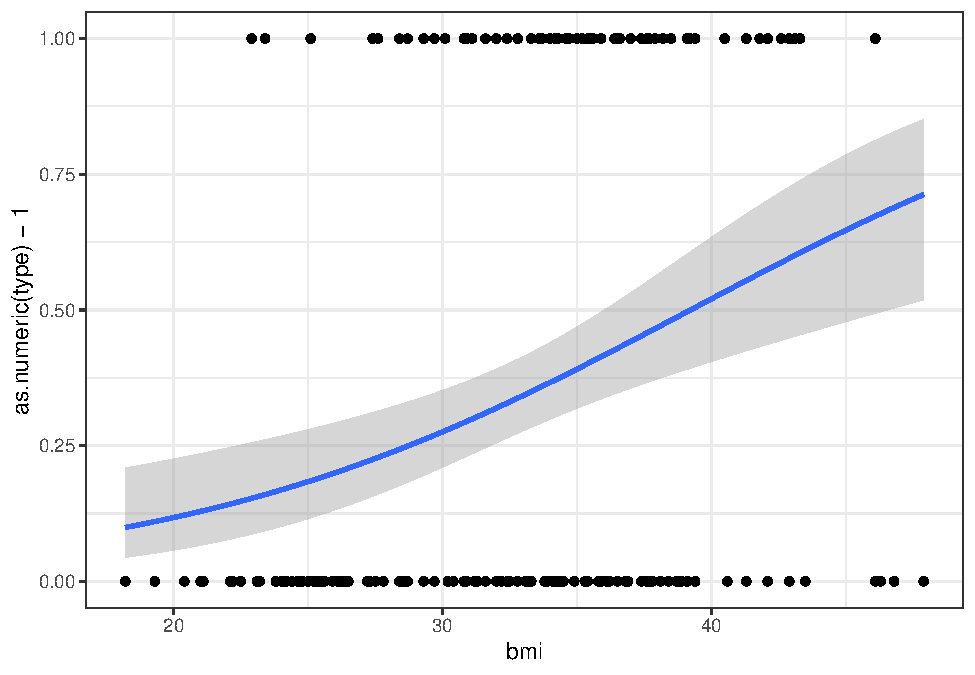
\includegraphics{bookglm_files/figure-latex/unnamed-chunk-4-1.pdf}

\begin{Shaded}
\begin{Highlighting}[]
\NormalTok{diabetes.model }\OtherTok{\textless{}{-}} \FunctionTok{glm}\NormalTok{(type}\SpecialCharTok{\textasciitilde{}}\NormalTok{bmi,}\AttributeTok{data=}\NormalTok{Pima.tr,}\AttributeTok{family=}\StringTok{"binomial"}\NormalTok{(}\AttributeTok{link=}\NormalTok{logit))}
\FunctionTok{summary}\NormalTok{(diabetes.model)}
\end{Highlighting}
\end{Shaded}

\begin{verbatim}
## 
## Call:
## glm(formula = type ~ bmi, family = binomial(link = logit), data = Pima.tr)
## 
## Deviance Residuals: 
##     Min       1Q   Median       3Q      Max  
## -1.5797  -0.9235  -0.6541   1.2506   1.9377  
## 
## Coefficients:
##             Estimate Std. Error z value Pr(>|z|)    
## (Intercept) -4.11156    0.92806  -4.430 9.41e-06 ***
## bmi          0.10482    0.02738   3.829 0.000129 ***
## ---
## Signif. codes:  0 '***' 0.001 '**' 0.01 '*' 0.05 '.' 0.1 ' ' 1
## 
## (Dispersion parameter for binomial family taken to be 1)
## 
##     Null deviance: 256.41  on 199  degrees of freedom
## Residual deviance: 239.97  on 198  degrees of freedom
## AIC: 243.97
## 
## Number of Fisher Scoring iterations: 4
\end{verbatim}

Si solo observa el valor \(p\), el resultado no sorprendente es que hay un relación entre el índice de masa corporal y la diabetes.

Profundizando en la salida con más detalle, nuestra ecuación de regresión logística es:

\[ ln(\frac{\hat{p}}{1-\hat{p}})=-4.11156+0.10482X \]

Suponga que queremos hacer una predicción para una mujer en esta población con un índice de masa corporal de \(X= 30\). Sustituya la ecuación para obtener su logit

\[
ln(\frac{\hat{p}}{1-\hat{p}})=-4.11156+0.10482(30)=-0.96696
\]

Observe que su logit (log odds-ratio) es negativo. Esto será cierto siempre que la probabilidad predicha \(\hat{p}<0.5\), por lo que en este escenario usted querría un logit negativo. Cuando \(\hat{p}>0.5\), el logit será positivo, y si \(\hat{p}= 0.5\) entonces el logit es::

\[
ln(\frac{0.5}{1-0.5})=ln(1)=0
\]
Probablemente preferiria una probabilidad o un porcentaje en lugar de un logit.Tome la funcion logit inversa para obtener esto.\\
\[\hat{p}=\frac{exp(-0.96696)}{1+exp(-0.96696)}=0.275 \]\\
Estamos pronosticando un \(27.5\%\) de probabilidad de diabetes tipo II cuando el índice de masa corporal es igual a \(X=30\).

Prestando atención al parámetro de ``pendiente'' \(\beta_1\), su estimación es \(0.10482\). Eso es positivo, lo que significa que bmi está asociado positivamente con el evento, que tiene diabetes tipo II. Por cada aumento de 1 unidad en X (es decir, alguien gana peso suficiente para que el bmi suba en 1), el aumento previsto en el logit es 0.10482.

Si esto no significa mucho para usted, entonces podemos exponencializar la pendiente para convertir el registro de la proporción de log probabilidades en solo la proporción de probabilidades.

\[exp(\hat{\beta_1})=e^{\hat{\beta_1}}=e^{0.10428}=1.11 \]
Entonces, la razón de posibilidades es \(1.11\). Esto significa que por cada aumento de 1 en el bmi, la probabilidad
de tener diabetes tipo II aumenta en un \(11\%\). Si la razón de posibilidades era exactamente 1, eso
indicaría una probabilidad igual (es decir, la variable no estaría asociada con la
evento), y las razones de probabilidad por debajo de 1 indican que la probabilidad disminuye a medida que la variable
aumenta. Si hubo un ejercicio de variable en el conjunto de datos que fue
asociado con tener diabetes, esperaríamos que su \(\beta\) fuera negativo, por lo que el
La razón de posibilidades estaría entre 0 y 1.

Si quisiéramos observar el impacto de un aumento de 10 puntos en el bmi (\(\Delta x=10\))

\(exp(\Delta x \hat{\beta_1} ) = exp(10\times 0.10428) = e^{1.0428} = 2.85\)\\
Las probabilidades(odss) de tener diabetes casi se triplicarían si el IMC aumenta en 10 unidades.

\hypertarget{test-de-wald-para-regresiuxf3n-loguxedstica}{%
\chapter{Test de Wald para regresión logística}\label{test-de-wald-para-regresiuxf3n-loguxedstica}}

R de forma predeterminada utiliza la prueba de Wald en la tabla de resumen para un lineal generalizado modelo. Repitamos esa tabla

\begin{Shaded}
\begin{Highlighting}[]
\FunctionTok{summary}\NormalTok{(diabetes.model)}
\end{Highlighting}
\end{Shaded}

\begin{verbatim}
## 
## Call:
## glm(formula = type ~ bmi, family = binomial(link = logit), data = Pima.tr)
## 
## Deviance Residuals: 
##     Min       1Q   Median       3Q      Max  
## -1.5797  -0.9235  -0.6541   1.2506   1.9377  
## 
## Coefficients:
##             Estimate Std. Error z value Pr(>|z|)    
## (Intercept) -4.11156    0.92806  -4.430 9.41e-06 ***
## bmi          0.10482    0.02738   3.829 0.000129 ***
## ---
## Signif. codes:  0 '***' 0.001 '**' 0.01 '*' 0.05 '.' 0.1 ' ' 1
## 
## (Dispersion parameter for binomial family taken to be 1)
## 
##     Null deviance: 256.41  on 199  degrees of freedom
## Residual deviance: 239.97  on 198  degrees of freedom
## AIC: 243.97
## 
## Number of Fisher Scoring iterations: 4
\end{verbatim}

R informa el estadístico de Wald \(z\), que es la raíz cuadrada de la prueba de Wald \(\chi^2\)
discutido en el capítulo 21. Esto se basa en el hecho matemático de que si
al cuadrado de la distribución normal estándar \(Z\), se obtiene una distribución chi-cuadrado
con \(df=1\).

Las hipótesis son:

\begin{equation}
H_0:\beta_{1}=0  \hspace{1cm} \textup{vs.}  \hspace{1cm} H_1:\beta_{1}\not= 0
\end{equation}

o en términos de odds-ratio \(\theta\)

\begin{equation}
H_0:\theta_{1}=0  \hspace{1cm} \textup{versus} \hspace{1cm} H_1:\theta_{1}\not= 0
\end{equation}

Observe que el estadístico \(z\) dado es la estimación dividida por el error estándar y el p-valor se basa en la distribución normal estándar.

\[z=\frac{\hat{\beta_1}}{S_{\hat{\beta_1}}}=\frac{0.10482}{0.02738}=3.849 \]

Existe una relación significativa entre bmi y diabetes tipo II:

Wald \(z=3.829\),\(p=0.000129\)

Algunos paquetes de software darán la prueba de chi-cuadrado de Wald en su lugar, que es solo nuestra estadística al cuadrado.

\[ \chi^2=\left(\frac{\hat{\beta_1}}{{S_{\beta_1}}}\right)^2=\left(\frac{0.10482}{0.02738}\right)^2=14.656\]
Dado que esta estadística es chi-cuadrado con \(df=1\), el valor de \(p\) es:

\begin{Shaded}
\begin{Highlighting}[]
\DecValTok{1}\SpecialCharTok{{-}}\FunctionTok{pchisq}\NormalTok{(}\FloatTok{14.656}\NormalTok{,}\AttributeTok{df=}\DecValTok{1}\NormalTok{)}
\end{Highlighting}
\end{Shaded}

\begin{verbatim}
## [1] 0.0001290233
\end{verbatim}

El intervalo de confianza de Wald para \(\beta_1\) se calcula de manera similar a muchos otros intervalos de confianza que hemos visto

\[\beta_1 \pm z(S_{\beta_1})\]

Para nuestro al \(95\%\) de confianza:

\[0.10482 \pm 1.96 \times 0.02738 \]\\
\[0.10482 \pm 0.05366 \]
\[\left( 0.05062,0.15794\right)\]

Exponencia este intervalo para obtener un intervalo de confianza para la razón de posibilidades \(\theta\)

\[\left(e^{0.05062}, e^{0.05062}\right) \]

Observe que el IC completo para \(\beta_1\) está por encima de cero y, de manera equivalente, el IC completo para \(\theta\) es
por encima de uno. Esto indica una relación significativa.

\hypertarget{prueba-de-razuxf3n-de-verosimilitud.}{%
\chapter{Prueba de razón de verosimilitud.}\label{prueba-de-razuxf3n-de-verosimilitud.}}

La inferencia para modelos lineales generalizados también se puede realizar con una razón de verosimilitud.

Esto implicará el análisis de la tabla de deviance.

\begin{Shaded}
\begin{Highlighting}[]
\FunctionTok{library}\NormalTok{(car)}
\end{Highlighting}
\end{Shaded}

\begin{verbatim}
## Loading required package: carData
\end{verbatim}

\begin{verbatim}
## 
## Attaching package: 'car'
\end{verbatim}

\begin{verbatim}
## The following objects are masked from 'package:mosaic':
## 
##     deltaMethod, logit
\end{verbatim}

\begin{verbatim}
## The following object is masked from 'package:psych':
## 
##     logit
\end{verbatim}

\begin{verbatim}
## The following object is masked from 'package:dplyr':
## 
##     recode
\end{verbatim}

\begin{verbatim}
## The following object is masked from 'package:purrr':
## 
##     some
\end{verbatim}

\begin{Shaded}
\begin{Highlighting}[]
\FunctionTok{Anova}\NormalTok{(diabetes.model,}\AttributeTok{type=}\StringTok{"II"}\NormalTok{,}\AttributeTok{test=}\StringTok{"LR"}\NormalTok{)}
\end{Highlighting}
\end{Shaded}

\begin{verbatim}
## Analysis of Deviance Table (Type II tests)
## 
## Response: type
##     LR Chisq Df Pr(>Chisq)    
## bmi   16.445  1  5.008e-05 ***
## ---
## Signif. codes:  0 '***' 0.001 '**' 0.01 '*' 0.05 '.' 0.1 ' ' 1
\end{verbatim}

Leyendo de la salida, vemos que \(\chi^2=16.445\) con \(df=1\), \(p< 0.0001\).

Observe que el estadístico de la prueba de chi cuadrado NO es igual al chi cuadrado de Wald prueba calculada anteriormente.

\[\chi^2=-2ln\left(\frac{\mathcal{L_R}}{\mathcal{L_F}}\right) \]

\[\chi^2=-2\left(ln\mathcal{L_R}-ln\mathcal{L_F}\right) \]
Hasta ahora, solo hemos ajustado el tipo de modelo completo type \textasciitilde{} bmi. Ajustemos el modelo reducido
escriba \textasciitilde{} 1 (es decir, un modelo de solo intercepción o ``nulo'') y calculamos las probabilidades logarítmicas y la deviance con R.

\begin{Shaded}
\begin{Highlighting}[]
\NormalTok{diabetes.null }\OtherTok{\textless{}{-}} \FunctionTok{glm}\NormalTok{(type}\SpecialCharTok{\textasciitilde{}}\DecValTok{1}\NormalTok{,}\AttributeTok{data=}\NormalTok{Pima.tr,}\AttributeTok{family=}\StringTok{"binomial"}\NormalTok{(}\AttributeTok{link=}\NormalTok{logit))}
\FunctionTok{logLik}\NormalTok{(diabetes.null)}
\end{Highlighting}
\end{Shaded}

\begin{verbatim}
## 'log Lik.' -128.2071 (df=1)
\end{verbatim}

\begin{Shaded}
\begin{Highlighting}[]
\FunctionTok{logLik}\NormalTok{(diabetes.model)}
\end{Highlighting}
\end{Shaded}

\begin{verbatim}
## 'log Lik.' -119.9846 (df=2)
\end{verbatim}

\begin{Shaded}
\begin{Highlighting}[]
\NormalTok{diff }\OtherTok{\textless{}{-}} \FunctionTok{logLik}\NormalTok{(diabetes.null)[}\DecValTok{1}\NormalTok{] }\SpecialCharTok{{-}} \FunctionTok{logLik}\NormalTok{(diabetes.model)[}\DecValTok{1}\NormalTok{]}
\NormalTok{chisq.LRT }\OtherTok{\textless{}{-}} \SpecialCharTok{{-}}\DecValTok{2}\SpecialCharTok{*}\NormalTok{diff}
\NormalTok{chisq.LRT}
\end{Highlighting}
\end{Shaded}

\begin{verbatim}
## [1] 16.44499
\end{verbatim}

\begin{Shaded}
\begin{Highlighting}[]
\NormalTok{pval.LRT }\OtherTok{\textless{}{-}} \DecValTok{1}\SpecialCharTok{{-}}\FunctionTok{pchisq}\NormalTok{(chisq.LRT,}\AttributeTok{df=}\DecValTok{1}\NormalTok{)}
\NormalTok{pval.LRT}
\end{Highlighting}
\end{Shaded}

\begin{verbatim}
## [1] 5.008242e-05
\end{verbatim}

Observe que obtenemos la misma estadística de prueba proporcionada por el comando Anova.
También mire nuevamente la parte inferior del resumen.

\begin{Shaded}
\begin{Highlighting}[]
\FunctionTok{summary}\NormalTok{(diabetes.model)}
\end{Highlighting}
\end{Shaded}

\begin{verbatim}
## 
## Call:
## glm(formula = type ~ bmi, family = binomial(link = logit), data = Pima.tr)
## 
## Deviance Residuals: 
##     Min       1Q   Median       3Q      Max  
## -1.5797  -0.9235  -0.6541   1.2506   1.9377  
## 
## Coefficients:
##             Estimate Std. Error z value Pr(>|z|)    
## (Intercept) -4.11156    0.92806  -4.430 9.41e-06 ***
## bmi          0.10482    0.02738   3.829 0.000129 ***
## ---
## Signif. codes:  0 '***' 0.001 '**' 0.01 '*' 0.05 '.' 0.1 ' ' 1
## 
## (Dispersion parameter for binomial family taken to be 1)
## 
##     Null deviance: 256.41  on 199  degrees of freedom
## Residual deviance: 239.97  on 198  degrees of freedom
## AIC: 243.97
## 
## Number of Fisher Scoring iterations: 4
\end{verbatim}

Observe que la diferencia de la desviación nula (256.41) y la desviación residual
(239.97) es 16.44, nuestro estadístico de prueba de chi-cuadrado con \(199-198 = 1df\) El
La desviación nula es -2 veces la forma logarítmica del modelo reducido, mientras que la
la desviación es -2 veces la probabilidad logarítmica del modelo completo. Esto es análogo a
el concepto de ``SS extra'' de las pruebas F parciales.

\hypertarget{regresiuxf3n-loguxedstica-muxfaltiple}{%
\chapter{REGRESIÓN LOGÍSTICA MÚLTIPLE}\label{regresiuxf3n-loguxedstica-muxfaltiple}}

Veamos cómo ajustar varios modelos de regresión logística a un conjunto de datos. Tomemos
el conjunto de datos Pima.tr y cree una variable categórica Mom donde una mujer
con npreg\textgreater{} 0 se clasifica como madre (sin tener en cuenta la posibilidad de que algunos
los embarazos pueden no haber resultado en un nacimiento vivo).

\begin{Shaded}
\begin{Highlighting}[]
\NormalTok{Pima.tr }\OtherTok{\textless{}{-}}\NormalTok{ Pima.tr }\SpecialCharTok{\%\textgreater{}\%}
\FunctionTok{mutate}\NormalTok{(}\AttributeTok{Mom=}\FunctionTok{ifelse}\NormalTok{(npreg}\SpecialCharTok{==}\DecValTok{0}\NormalTok{,}\StringTok{"No"}\NormalTok{,}\StringTok{"Yes"}\NormalTok{))}
\FunctionTok{xtabs}\NormalTok{(}\SpecialCharTok{\textasciitilde{}}\NormalTok{type}\SpecialCharTok{+}\NormalTok{Mom,}\AttributeTok{data=}\NormalTok{Pima.tr)}
\end{Highlighting}
\end{Shaded}

\begin{verbatim}
##      Mom
## type   No Yes
##   No   16 116
##   Yes  12  56
\end{verbatim}

Calculemos la razón de posibilidades(odss-ratio) de la tabla :

\[ OR=\dfrac{\frac{a}{b}}{\frac{c}{d}}=\dfrac{\frac{16}{116}}{\frac{12}{256}}=0.6437\]
Tomaremos el recíproco para facilitar la interpretación, \(\frac{1}{OR}=\frac{1}{0.6437}=1.5536\)

Las probabilidades
de tener diabetes tipo II son 1.55 veces mayores para las no madres que para las madres.
Observe que aproximadamente el \(43\%\) de las no madres y el\\
\(33\%\) de las madres tienen el Tipo II diabetes.

Primero, encuentre un intervalo de confianza para el logaritmo de la razón de posibilidades(logit)

\[ln(OR)\pm z\sqrt{\frac{1}{a}+\frac{1}{b}+\frac{1}{c}+\frac{1}{d} }\]
\[ln(1.5536)\pm (1.96)\sqrt{\frac{1}{16}+\frac{1}{116}+\frac{1}{12}+\frac{1}{56}} \]

\[\left( 0.4406 \pm 0.8316\right) \]
\[(-0.3730, 1.2542)\]

Este intervalo de confianza contiene 0, por lo que la variable Mom no es un predictor significativo
de la diabetes tipo II. Si prefiere el IC en términos de razón de posibilidades, exponencial.

\[ \left( e^{-0.3730} , e^{1.2542}\right) \]

\[\left( 0.6887, 3.5050\right) \]

El IC incluye el valor 1 (que indica que no hay efecto para la razón de posibilidades).

Usemos R para ajustar el tipo de type\textasciitilde Mom

\begin{Shaded}
\begin{Highlighting}[]
\NormalTok{mod0}\OtherTok{\textless{}{-}} \FunctionTok{glm}\NormalTok{(type}\SpecialCharTok{\textasciitilde{}}\DecValTok{1}\NormalTok{,}\AttributeTok{data=}\NormalTok{Pima.tr,}\AttributeTok{family=}\StringTok{"binomial"}\NormalTok{(}\AttributeTok{link=}\NormalTok{logit))}
\NormalTok{mod1}\OtherTok{\textless{}{-}} \FunctionTok{glm}\NormalTok{(type}\SpecialCharTok{\textasciitilde{}}\NormalTok{Mom,}\AttributeTok{data=}\NormalTok{Pima.tr,}\AttributeTok{family=}\StringTok{"binomial"}\NormalTok{(}\AttributeTok{link=}\NormalTok{logit))}
\FunctionTok{summary}\NormalTok{(mod1)}
\end{Highlighting}
\end{Shaded}

\begin{verbatim}
## 
## Call:
## glm(formula = type ~ Mom, family = binomial(link = logit), data = Pima.tr)
## 
## Deviance Residuals: 
##     Min       1Q   Median       3Q      Max  
## -1.0579  -0.8876  -0.8876   1.4981   1.4981  
## 
## Coefficients:
##             Estimate Std. Error z value Pr(>|z|)
## (Intercept)  -0.2877     0.3819  -0.753    0.451
## MomYes       -0.4406     0.4151  -1.061    0.289
## 
## (Dispersion parameter for binomial family taken to be 1)
## 
##     Null deviance: 256.41  on 199  degrees of freedom
## Residual deviance: 255.31  on 198  degrees of freedom
## AIC: 259.31
## 
## Number of Fisher Scoring iterations: 4
\end{verbatim}

\begin{Shaded}
\begin{Highlighting}[]
\FunctionTok{Anova}\NormalTok{(mod1,}\AttributeTok{test=}\StringTok{"LR"}\NormalTok{)}
\end{Highlighting}
\end{Shaded}

\begin{verbatim}
## Analysis of Deviance Table (Type II tests)
## 
## Response: type
##     LR Chisq Df Pr(>Chisq)
## Mom   1.1056  1     0.2931
\end{verbatim}

\begin{Shaded}
\begin{Highlighting}[]
\FunctionTok{confint}\NormalTok{(mod1)}
\end{Highlighting}
\end{Shaded}

\begin{verbatim}
## Waiting for profiling to be done...
\end{verbatim}

\begin{verbatim}
##                 2.5 %    97.5 %
## (Intercept) -1.058545 0.4561131
## MomYes      -1.250578 0.3907974
\end{verbatim}

Vemos que Mom no es significativa con la prueba de Wald o la razón de verosimilitud
prueba. El intervalo de confianza se calcula con una fórmula más compleja que
dado aquí, por lo que los resultados no son idénticos. Los signos son opuestos porque mi
La tabla usó \textbf{No} como un éxito y el ajuste glm de R usó \textbf{Sí} como un éxito.
Hagamos una regresión logística múltiple y hagamos una predicción. Usaré 3 predictores
bmi, age y Mom.

\begin{Shaded}
\begin{Highlighting}[]
\NormalTok{mod2 }\OtherTok{\textless{}{-}} \FunctionTok{glm}\NormalTok{(type}\SpecialCharTok{\textasciitilde{}}\NormalTok{bmi}\SpecialCharTok{+}\NormalTok{age}\SpecialCharTok{+}\NormalTok{Mom,}\AttributeTok{data=}\NormalTok{Pima.tr,}\AttributeTok{family=}\StringTok{"binomial"}\NormalTok{(}\AttributeTok{link=}\NormalTok{logit))}
\FunctionTok{summary}\NormalTok{(mod2)}
\end{Highlighting}
\end{Shaded}

\begin{verbatim}
## 
## Call:
## glm(formula = type ~ bmi + age + Mom, family = binomial(link = logit), 
##     data = Pima.tr)
## 
## Deviance Residuals: 
##     Min       1Q   Median       3Q      Max  
## -1.8477  -0.8045  -0.4907   0.9983   2.3009  
## 
## Coefficients:
##             Estimate Std. Error z value Pr(>|z|)    
## (Intercept) -5.76192    1.23679  -4.659 3.18e-06 ***
## bmi          0.09703    0.03011   3.223  0.00127 ** 
## age          0.07830    0.01628   4.809 1.52e-06 ***
## MomYes      -0.83471    0.48052  -1.737  0.08237 .  
## ---
## Signif. codes:  0 '***' 0.001 '**' 0.01 '*' 0.05 '.' 0.1 ' ' 1
## 
## (Dispersion parameter for binomial family taken to be 1)
## 
##     Null deviance: 256.41  on 199  degrees of freedom
## Residual deviance: 212.96  on 196  degrees of freedom
## AIC: 220.96
## 
## Number of Fisher Scoring iterations: 4
\end{verbatim}

Observe que el bmi y la edad son predictores significativos de bmi con valores pendiente positivas.
Lo que indica un mayor riesgo a medida que aumenta el bmi o la edad. Mom no es
significativo en \(\alpha=0.05\), pero tiene una pendiente negativa que indica que las madres fueron menos probabilidades de ser diabéticas que las no madres.

Si una mujer tiene 40 años, un bmi de 28 y es madre, calculemos su
probabilidad de diabetes tipo II.

\[ln\left(\frac{\hat{\pi}}{1-\hat{\pi}}\right)=-5.76192 + 0.09703(28) + 0.07830(40)-0.83471(1) = -0.74779 \]

Su logit negativo indica menos del \(50\%\) de posibilidades de diabetes. Tomando el logit inverso:

\[\frac{e^{-0.74779}}{1+e^{-0.74779}}=0.321 \]

La probabilidad es de aproximadamente el \(32\%\). Ahora hazlo para una persona con las mismas estadísticas,
excepto que no sea madre.

\[ ln\left(\frac{\hat{\pi}}{1-\hat{\pi}}\right)=-5.76192 + 0.09703(28) + 0.07830(40)-0.83471(0) = 0.08692\]

Ahora el logit es positivo, por lo que la probabilidad será superior al \(50\%\).

\[\frac{e^{0.08692}}{1+e^{0.08692}}=0.522 \]

Una prueba de razón de verosimilitud que compara el modelo 1 (solo con mamá) y el modelo 2 (con
bmi, age y Mom) tendrá \(df=2\) con dos parámetros adicionales, y tendríamos esperar que el segundo modelo sea una mejora significativa.

\begin{Shaded}
\begin{Highlighting}[]
\FunctionTok{anova}\NormalTok{(mod1,mod2,}\AttributeTok{test=}\StringTok{"LR"}\NormalTok{)}
\end{Highlighting}
\end{Shaded}

\begin{verbatim}
## Analysis of Deviance Table
## 
## Model 1: type ~ Mom
## Model 2: type ~ bmi + age + Mom
##   Resid. Df Resid. Dev Df Deviance  Pr(>Chi)    
## 1       198     255.31                          
## 2       196     212.96  2   42.353 6.355e-10 ***
## ---
## Signif. codes:  0 '***' 0.001 '**' 0.01 '*' 0.05 '.' 0.1 ' ' 1
\end{verbatim}

Vemos que hay una mejora significativa, con \(\chi^2=42.353\), \(df=2\) y \(p=0.0001\).

Tal vez no deberíamos haber creado una variable categórica como Mom, pero solo usar
npreg. Encajaré un tercer tipo de type \textasciitilde{} bmi + age + npreg.

\begin{Shaded}
\begin{Highlighting}[]
\NormalTok{mod3 }\OtherTok{\textless{}{-}} \FunctionTok{glm}\NormalTok{(type}\SpecialCharTok{\textasciitilde{}}\NormalTok{bmi}\SpecialCharTok{+}\NormalTok{age}\SpecialCharTok{+}\NormalTok{npreg,}\AttributeTok{data=}\NormalTok{Pima.tr,}\AttributeTok{family=}\StringTok{"binomial"}\NormalTok{(}\AttributeTok{link=}\NormalTok{logit))}
\FunctionTok{summary}\NormalTok{(mod3)}
\end{Highlighting}
\end{Shaded}

\begin{verbatim}
## 
## Call:
## glm(formula = type ~ bmi + age + npreg, family = binomial(link = logit), 
##     data = Pima.tr)
## 
## Deviance Residuals: 
##     Min       1Q   Median       3Q      Max  
## -1.7413  -0.8235  -0.4918   0.9773   2.2382  
## 
## Coefficients:
##             Estimate Std. Error z value Pr(>|z|)    
## (Intercept) -6.44462    1.18360  -5.445 5.18e-08 ***
## bmi          0.10761    0.02986   3.604 0.000313 ***
## age          0.05937    0.01817   3.267 0.001086 ** 
## npreg        0.06508    0.05720   1.138 0.255226    
## ---
## Signif. codes:  0 '***' 0.001 '**' 0.01 '*' 0.05 '.' 0.1 ' ' 1
## 
## (Dispersion parameter for binomial family taken to be 1)
## 
##     Null deviance: 256.41  on 199  degrees of freedom
## Residual deviance: 214.62  on 196  degrees of freedom
## AIC: 222.62
## 
## Number of Fisher Scoring iterations: 4
\end{verbatim}

Algo extraño, ya que npreg no es significativo, pero el signo de su estimación es positivo,
en lugar de negativo para Mom. Puede haber alguna explicación médica. No soy
conciente de.

Por último, suponga que quisiera comparar los modelos 2 y 3. No están anidados, por lo que
necesita usar AIC en su lugar. Crearé una tabla AIC para los cuatro modelos (incluidos el modelo nulo).

\begin{Shaded}
\begin{Highlighting}[]
\FunctionTok{require}\NormalTok{(bbmle)}
\end{Highlighting}
\end{Shaded}

\begin{verbatim}
## Loading required package: bbmle
\end{verbatim}

\begin{verbatim}
## Loading required package: stats4
\end{verbatim}

\begin{verbatim}
## 
## Attaching package: 'bbmle'
\end{verbatim}

\begin{verbatim}
## The following object is masked from 'package:dplyr':
## 
##     slice
\end{verbatim}

\begin{Shaded}
\begin{Highlighting}[]
\FunctionTok{AICtab}\NormalTok{(mod0,mod1,mod2,mod3,}\AttributeTok{base=}\ConstantTok{TRUE}\NormalTok{,}\AttributeTok{delta=}\ConstantTok{TRUE}\NormalTok{,}\AttributeTok{weights=}\ConstantTok{TRUE}\NormalTok{,}\AttributeTok{sort=}\ConstantTok{TRUE}\NormalTok{)}
\end{Highlighting}
\end{Shaded}

\begin{verbatim}
##      AIC   dAIC  df weight
## mod2 221.0   0.0 4  0.7   
## mod3 222.6   1.7 4  0.3   
## mod0 258.4  37.5 1  <0.001
## mod1 259.3  38.4 2  <0.001
\end{verbatim}

Al AIC parece gustarle un poco más el Model 2 que el Model 3, aunque no hasta cierto punto
eso se consideraría sustancial. El modelo 0 y el modelo 1 son muy débiles, con \(\Delta_i>10\) y pesos diminutos Akaike \(w_i<0.001\).

\begin{Shaded}
\begin{Highlighting}[]
\FunctionTok{predict}\NormalTok{(}\AttributeTok{object =}\NormalTok{ mod2, }\AttributeTok{newdata =} \FunctionTok{data.frame}\NormalTok{(}\AttributeTok{bmi =}\FloatTok{30.3}\NormalTok{ ,}\AttributeTok{age=}\DecValTok{27}\NormalTok{,}\AttributeTok{Mom=}\StringTok{"No"}\NormalTok{))}
\end{Highlighting}
\end{Shaded}

\begin{verbatim}
##          1 
## -0.7077035
\end{verbatim}

\hypertarget{regresiuxf3n-de-poisson}{%
\chapter{Regresión de Poisson}\label{regresiuxf3n-de-poisson}}

\hypertarget{quuxe9-son-los-modelos-de-regresiuxf3n-de-poisson}{%
\section{¿Qué son los modelos de regresión de Poisson?}\label{quuxe9-son-los-modelos-de-regresiuxf3n-de-poisson}}

Los modelos de \emph{regresión de Poisson} se utilizan mejor para modelar eventos en los que se cuentan los resultados. O, más específicamente, contar datos: datos discretos con valores enteros no negativos que cuentan algo, como la cantidad de veces que ocurre un evento durante un período de tiempo determinado o la cantidad de personas en la fila en la tienda de comestibles.

Los datos de recuento también se pueden expresar como datos de tasa, ya que el número de veces que ocurre un evento dentro de un período de tiempo se puede expresar como una cuenta sin procesar (es decir, ``En un día, comemos tres comidas'') o como una tasa (``Comemos a una tasa de 0,125 comidas por hora'').

\textbf{La regresión de Poisson} nos ayuda a analizar tanto los datos de recuento como los datos de tasa al permitirnos determinar qué variables explicativas (valores X) tienen un efecto en una variable de respuesta dada (valor Y, el recuento o una tasa). Por ejemplo, una tienda de comestibles podría aplicar la regresión de Poisson para comprender y predecir mejor la cantidad de personas en una línea.

\hypertarget{en-quuxe9-se-diferencia-la-distribuciuxf3n-de-poisson-de-la-distribuciuxf3n-normal}{%
\section{¿En qué se diferencia la distribución de Poisson de la distribución normal?}\label{en-quuxe9-se-diferencia-la-distribuciuxf3n-de-poisson-de-la-distribuciuxf3n-normal}}

La distribución de Poisson se usa más comúnmente para encontrar la probabilidad de que ocurran eventos dentro de un intervalo de tiempo dado. Dado que estamos hablando de un recuento, con la distribución de Poisson, el resultado debe ser 0 o superior; no es posible que un evento ocurra un número negativo de veces. Por otro lado, la distribución normal es una distribución continua para una variable continua y podría resultar en un valor positivo o negativo:

\begin{longtable}[]{@{}
  >{\raggedright\arraybackslash}p{(\columnwidth - 2\tabcolsep) * \real{0.39}}
  >{\raggedright\arraybackslash}p{(\columnwidth - 2\tabcolsep) * \real{0.61}}@{}}
\toprule
Distribución Poisson & Distribución Normal \\
\midrule
\endhead
Se utiliza para contar datos o tasa(razón) de datos. & Usada para variables contínuas \\
Sesgada según los valores de lambda & Curva en forma de campana que es simétrica alrededor de la media \\
Varianza igual que la media & La varianza y la media son parámetros diferentes; media, mediana y moda son iguales \\
& \\
\bottomrule
\end{longtable}

Podemos generar una distribución normal en R así:

\begin{Shaded}
\begin{Highlighting}[]
\CommentTok{\# create a sequence {-}3 to +3 with .05 increments}
\NormalTok{xseq}\OtherTok{\textless{}{-}}\FunctionTok{seq}\NormalTok{(}\SpecialCharTok{{-}}\DecValTok{3}\NormalTok{, }\DecValTok{3}\NormalTok{, .}\DecValTok{05}\NormalTok{) }
\CommentTok{\# generate a Probability Density Function}
\NormalTok{densities }\OtherTok{\textless{}{-}} \FunctionTok{dnorm}\NormalTok{(xseq, }\DecValTok{0}\NormalTok{, }\DecValTok{1}\NormalTok{)}
\CommentTok{\# plot the graph}
\FunctionTok{plot}\NormalTok{(xseq, densities, }\AttributeTok{col =} \StringTok{"blue"}\NormalTok{, }\AttributeTok{xlab =} \StringTok{""}\NormalTok{, }\AttributeTok{ylab =} \StringTok{"Density"}\NormalTok{, }\AttributeTok{type =} \StringTok{"l"}\NormalTok{, }\AttributeTok{lwd =} \DecValTok{2}\NormalTok{)}
\end{Highlighting}
\end{Shaded}

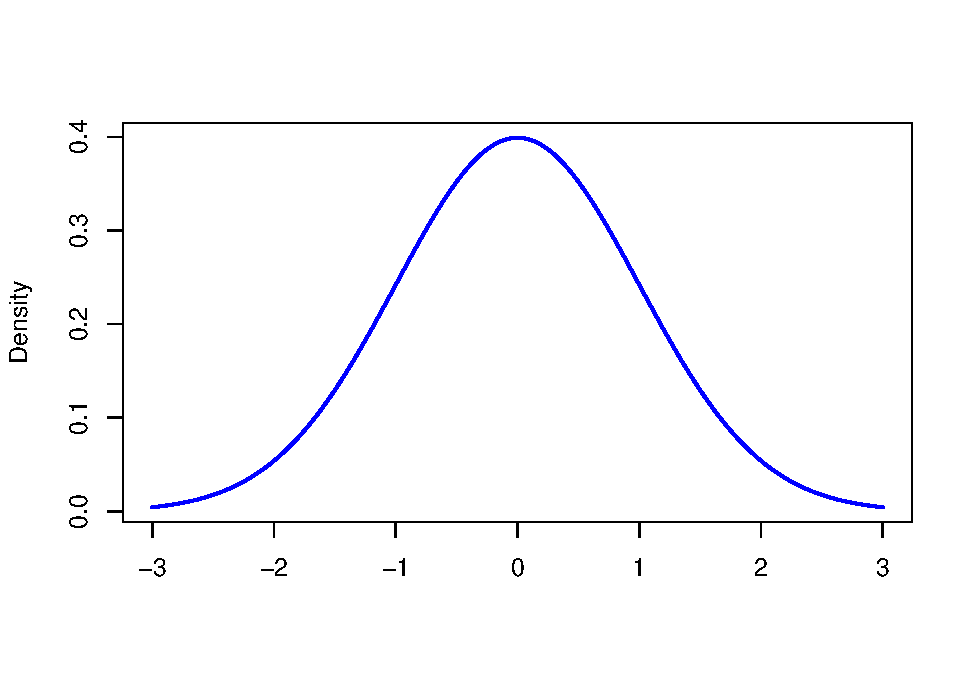
\includegraphics{bookglm_files/figure-latex/unnamed-chunk-23-1.pdf}

\begin{Shaded}
\begin{Highlighting}[]
\CommentTok{\# col: changes the color of line}
\CommentTok{\# \textquotesingle{}xlab\textquotesingle{} and \textquotesingle{}ylab\textquotesingle{} are labels for x and y axis respectively}
\CommentTok{\# type: defines the type of plot. \textquotesingle{}l\textquotesingle{} gives a line graph}
\CommentTok{\# lwd: defines line width}
\end{Highlighting}
\end{Shaded}

En R, \textbf{dnorm (secuencia, media, std.dev)} se usa para trazar la función de densidad de probabilidad (PDF) de una distribución normal.

Para comprender la distribución de Poisson, considere el siguiente problema del libro de texto Tutorial R de Chi Yau:

\textbf{Si hay 12 automóviles que cruzan un puente por minuto en promedio, ¿cuál es la probabilidad de que diecisiete o más automóviles crucen el puente en un minuto dado?}

Aquí, la cantidad promedio de automóviles que cruzan un puente por minuto es \(\mu=12\).

\texttt{ppois(q,\ u,\ lower.tail\ =\ TRUE)} es una función R que da la probabilidad de que una variable aleatoria sea menor o igual a un valor.

Tenemos que encontrar la probabilidad de tener diecisiete o más autos, por lo que usaremos \texttt{lower.trail\ =\ FALSE} y estableceremos q en 16:

\begin{Shaded}
\begin{Highlighting}[]
\FunctionTok{ppois}\NormalTok{(}\DecValTok{16}\NormalTok{, }\DecValTok{12}\NormalTok{, }\AttributeTok{lower.tail =} \ConstantTok{FALSE}\NormalTok{)}
\end{Highlighting}
\end{Shaded}

\begin{verbatim}
## [1] 0.101291
\end{verbatim}

\begin{Shaded}
\begin{Highlighting}[]
\CommentTok{\# lower.tail = logical; if TRUE (default) then probabilities are P[X \textless{} = x], otherwise, P[X \textgreater{} x].}
\end{Highlighting}
\end{Shaded}

Para obtener un porcentaje, simplemente necesitamos multiplicar esta salida por 100. Ahora tenemos la respuesta a nuestra pregunta: hay una probabilidad del \(10.1\%\) de tener 17 o más autos cruzando el puente en cualquier minuto en particular.

\hypertarget{modelos-de-regresiuxf3n-de-poisson-y-glmgeneralized-linear-models}{%
\section{Modelos de regresión de Poisson y GLM(Generalized Linear MOdels)}\label{modelos-de-regresiuxf3n-de-poisson-y-glmgeneralized-linear-models}}

Los modelos lineales generalizados son modelos en los que las variables de respuesta siguen una distribución diferente a la distribución normal. Eso contrasta con los modelos de regresión lineal, en los que las variables de respuesta siguen una distribución normal. Esto se debe a que los modelos lineales generalizados tienen variables de respuesta que son categóricas, como Sí, No; o Grupo A, Grupo B y, por lo tanto, no van de \(\infty\) a \(\infty\). Por tanto, la relación entre la respuesta y las variables predictoras puede no ser lineal. En GLM

\(y_i=\alpha+\beta_1X_{1i}+\beta_2X_{2i}+\ldots+\beta_pX_{pi}+e_i\), \vspace{1cm}\(i=1,2,\ldots,n\)

La variable de respuesta \(y_i\) se modela mediante una función lineal de variables predictoras y algún término de error.

Un \textbf{modelo de regresión de Poisson} es un modelo lineal generalizado (GLM) que se utiliza para modelar datos de recuento y tablas de contingencia. La salida \(Y\) (recuento) es un valor que sigue la distribución de Poisson. Asume el logaritmo de los valores esperados (media) que pueden modelarse en forma lineal mediante algunos parámetros desconocidos.

Para transformar la relación no lineal en forma lineal, se utiliza una función de enlace que es el logaritmo de la regresión de Poisson. Por esa razón, un modelo de regresión de Poisson también se denomina modelo log-lineal. La forma matemática general del modelo de regresión de Poisson es:

\[log(y)=\alpha +\beta_1X_1+\beta_2X_2+\cdots+\beta_pX_p\]

donde,

\begin{itemize}
\item
  \(y\) es la variable respuesta
\item
  \(\alpha\) y \(\beta\): son coeficientes numéricos, \(\alpha\) es la intersección, a veces \(\alpha\) también está representada por \(\beta_0\), es lo mismo.
\item
  x es la variable predictora/explicativa
\end{itemize}

Los coeficientes se calculan utilizando métodos como la \textbf{Estimación de máxima verosimilitud (MLE)} o la cuasi-verosimilitud máxima.

Considere una ecuación con una variable predictora y una variable de respuesta:

\[log(y)=\alpha+\beta(x) \]

Esto es equivalente a,

\[y=e^{\alpha+\beta X} \]

\textbf{Nota:} En los modelos de regresión de Poisson, las variables predictoras o explicativas pueden tener una combinación de valores numéricos o categóricos.

Una de las características más importantes para la distribución de Poisson y la regresión de Poisson es la equidispersión, lo que significa que la media y la varianza de la distribución son iguales.

La varianza mide la dispersión de los datos. Es el ``promedio de las diferencias al cuadrado de la media''. La varianza (Var) es igual a 0 si todos los valores son idénticos. Cuanto mayor sea la diferencia entre los valores, mayor será la varianza. La media es el promedio de valores de un conjunto de datos. El promedio es la suma de los valores dividida por el número de valores.

Digamos que la media (\(\mu\)) se denota por \(E(X)\)

\[E(X)=\mu\] Para la regresión de Poisson, la media y la varianza se relacionan como:

\[var(X)=\sigma^2E(X) \] Donde \(\sigma^2\) es el parámetro de Dispersión.

Dado que \(var(X)=E(X)\) (varianza = media) debe ser válida para que el modelo de Poisson se ajuste completamente, \(\sigma^2\) debe ser igual a 1.

Cuando la varianza es mayor que la media, eso se denomina sobredispersión y es mayor que 1. Si es menor que 1, se conoce como subdispersión.

\hypertarget{modelado-de-regresiuxf3n-de-poisson-utilizando-datos-de-recuento.}{%
\section{Modelado de regresión de Poisson utilizando datos de recuento.}\label{modelado-de-regresiuxf3n-de-poisson-utilizando-datos-de-recuento.}}

En R, el comando \texttt{glm\ ()}se usa para modelar modelos lineales generalizados. Aquí está la estructura general de \texttt{glm\ ()}:

\begin{verbatim}
glm(formula, family = familytype(link = ""), data,...)
\end{verbatim}

\textbf{formula} La fórmula es una representación simbólica de cómo se modela para ajustar.

\textbf{family} La familia indica la elección de las funciones de varianza y enlace. Hay varias opciones de familia, incluidas Poisson y Logistic.

\textbf{datos} Los datos son el conjunto de datos que se utilizará.

\texttt{glm()} ofrece ocho opciones para la familia con las siguientes funciones de enlace predeterminadas:

\begin{longtable}[]{@{}
  >{\raggedright\arraybackslash}p{(\columnwidth - 2\tabcolsep) * \real{0.26}}
  >{\raggedright\arraybackslash}p{(\columnwidth - 2\tabcolsep) * \real{0.62}}@{}}
\toprule
\textbf{Family} & \textbf{Default Link Function} \\
\midrule
\endhead
binomial & (link = ``logit'') \\
gaussian & (link = ``identity'') \\
Gamma & (link = ``inverse'') \\
inverse.gaussian & (link = \$frac\{1\}\{mu\^{}2\}\$) \\
poisson & \vtop{\hbox{\strut }\hbox{\strut (link = ``log'')}} \\
quasi & (link = ``identity'', variance = ``constant'') \\
quasibinomial & \vtop{\hbox{\strut }\hbox{\strut (link = ``logit'')}} \\
quasipoisson & (link = ``log'') \\
& \\
\bottomrule
\end{longtable}

\hypertarget{empecemos-a-modelar}{%
\subsection{¡Empecemos a modelar!}\label{empecemos-a-modelar}}

Vamos a modelar la regresión de Poisson relacionada con la frecuencia con la que el hilo se rompe durante el tejido. Estos datos se encuentran en el paquete \textbf{\texttt{datasets}} en R, por lo que lo primero que debemos hacer es instalar el paquete usando \texttt{install.packages("datasets")} y cargar la biblioteca con la librería \texttt{library(datasets):}

\begin{Shaded}
\begin{Highlighting}[]
\CommentTok{\# install.packages("datasets")}
\FunctionTok{library}\NormalTok{(datasets) }\CommentTok{\# include library datasets after installation}
\end{Highlighting}
\end{Shaded}

El paquete\texttt{datasets}incluye toneladas de conjuntos de datos, por lo que debemos seleccionar específicamente nuestros datos de hilo(yarn). \href{https://cran.r-project.org/manuals.html}{Consultando la documentación del paquete}, podemos ver que se llama \texttt{warpbreaks}, así que almacenémoslo como un objeto.

\begin{Shaded}
\begin{Highlighting}[]
\NormalTok{data}\OtherTok{\textless{}{-}}\NormalTok{warpbreaks}
\FunctionTok{head}\NormalTok{(data,}\DecValTok{10}\NormalTok{)}
\end{Highlighting}
\end{Shaded}

\begin{verbatim}
##    breaks wool tension
## 1      26    A       L
## 2      30    A       L
## 3      54    A       L
## 4      25    A       L
## 5      70    A       L
## 6      52    A       L
## 7      51    A       L
## 8      26    A       L
## 9      67    A       L
## 10     18    A       M
\end{verbatim}

Echemos un vistaso a los datos:

\begin{Shaded}
\begin{Highlighting}[]
\NormalTok{columns}\OtherTok{\textless{}{-}}\FunctionTok{names}\NormalTok{(data) }\CommentTok{\# Extract column names from dataframe}
\NormalTok{columns }\CommentTok{\# show columns}
\end{Highlighting}
\end{Shaded}

\begin{verbatim}
## [1] "breaks"  "wool"    "tension"
\end{verbatim}

\textbf{¿Qué hay en nuestros datos?}

Este conjunto de datos analiza cuántas roturas de urdimbre ocurrieron para diferentes tipos de telares por telar, por longitud fija de hilo. Podemos leer más detalles sobre este conjunto de datos en la documentación \href{https://cran.r-project.org/manuals.html}{aquí}, pero aquí están las tres columnas que veremos y a qué se refiere cada una:

\begin{longtable}[]{@{}lll@{}}
\toprule
Variable & Tipo & Descripción \\
\midrule
\endhead
breaks & numérica & número de roturas \\
wool & factor & El tipo de lana(A o B) \\
tension & factor & El nivel de tensión (L, M, H) \\
& & \\
\bottomrule
\end{longtable}

Hay medidas en 9 telares de cada uno de los seis tipos de deformación, para un total de 54 entradas en el conjunto de datos.

Veamos cómo se estructuran los datos mediante el comando\texttt{ls.str\ ():}

\begin{Shaded}
\begin{Highlighting}[]
\FunctionTok{ls.str}\NormalTok{(warpbreaks)}
\end{Highlighting}
\end{Shaded}

\begin{verbatim}
## breaks :  num [1:54] 26 30 54 25 70 52 51 26 67 18 ...
## tension :  Factor w/ 3 levels "L","M","H": 1 1 1 1 1 1 1 1 1 2 ...
## wool :  Factor w/ 2 levels "A","B": 1 1 1 1 1 1 1 1 1 1 ...
\end{verbatim}

De lo anterior, podemos ver tanto los tipos como los niveles presentes en los datos. Lea \href{https://www.statmethods.net/input/datatypes.html}{esto} para aprender un poco más sobre los factores en R.

Ahora trabajaremos con el marco de datos. Recuerde, con un modelo de distribución de Poisson estamos tratando de averiguar cómo algunas variables predictoras afectan una variable de respuesta. Aquí, \texttt{breaks} es la variable de respuesta y \texttt{wool} y \texttt{tension} son variables predictoras.

Podemos ver que la variable dependiente breaks de datos contínuos creando un histograma:

\begin{Shaded}
\begin{Highlighting}[]
\FunctionTok{hist}\NormalTok{(data}\SpecialCharTok{$}\NormalTok{breaks)}
\end{Highlighting}
\end{Shaded}

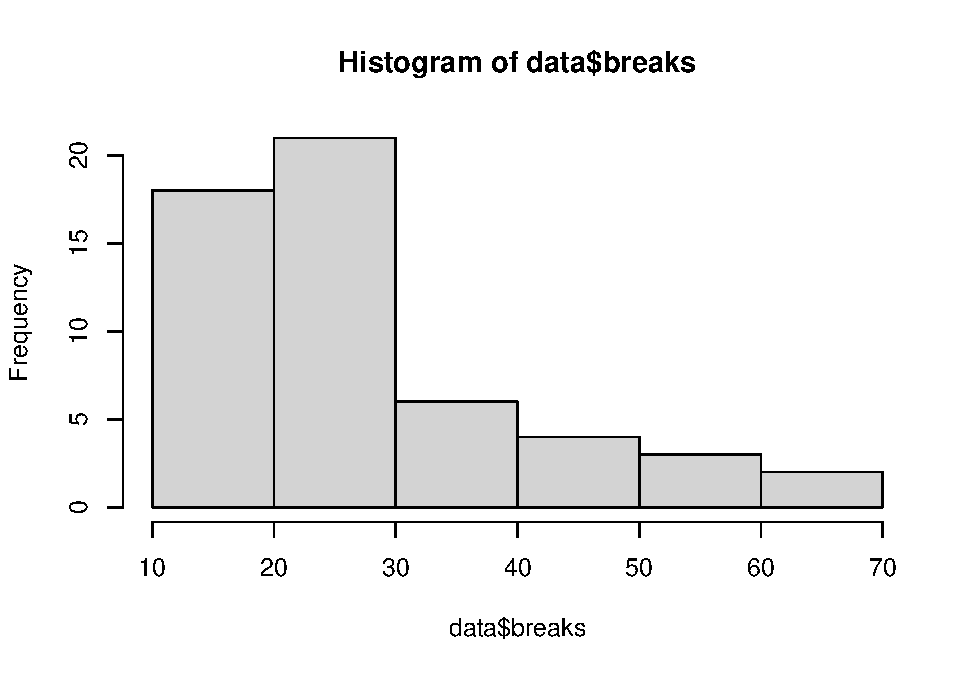
\includegraphics{bookglm_files/figure-latex/unnamed-chunk-29-1.pdf}

Claramente, los datos no tienen la forma de una curva de campana como en una distribución normal.

Veamos la media \texttt{mean()}y la varianza \texttt{var\ ()}de la variable dependiente:

\begin{Shaded}
\begin{Highlighting}[]
\FunctionTok{mean}\NormalTok{(data}\SpecialCharTok{$}\NormalTok{breaks) }\CommentTok{\# calculate mean}
\end{Highlighting}
\end{Shaded}

\begin{verbatim}
## [1] 28.14815
\end{verbatim}

\begin{Shaded}
\begin{Highlighting}[]
\FunctionTok{var}\NormalTok{(data}\SpecialCharTok{$}\NormalTok{breaks) }\CommentTok{\# calculate variance}
\end{Highlighting}
\end{Shaded}

\begin{verbatim}
## [1] 174.2041
\end{verbatim}

La varianza es mucho mayor que la media, lo que sugiere que tendremos una dispersión excesiva en el modelo.

Ajustemos el modelo de Poisson usando el comando \texttt{glm\ ().}

\begin{Shaded}
\begin{Highlighting}[]
\CommentTok{\# model poisson regression using glm()}
\NormalTok{poisson.model}\OtherTok{\textless{}{-}}\FunctionTok{glm}\NormalTok{(breaks }\SpecialCharTok{\textasciitilde{}}\NormalTok{ wool }\SpecialCharTok{+}\NormalTok{ tension, data, }\AttributeTok{family =} \FunctionTok{poisson}\NormalTok{(}\AttributeTok{link =} \StringTok{"log"}\NormalTok{))}
\FunctionTok{summary}\NormalTok{(poisson.model)}
\end{Highlighting}
\end{Shaded}

\begin{verbatim}
## 
## Call:
## glm(formula = breaks ~ wool + tension, family = poisson(link = "log"), 
##     data = data)
## 
## Deviance Residuals: 
##     Min       1Q   Median       3Q      Max  
## -3.6871  -1.6503  -0.4269   1.1902   4.2616  
## 
## Coefficients:
##             Estimate Std. Error z value Pr(>|z|)    
## (Intercept)  3.69196    0.04541  81.302  < 2e-16 ***
## woolB       -0.20599    0.05157  -3.994 6.49e-05 ***
## tensionM    -0.32132    0.06027  -5.332 9.73e-08 ***
## tensionH    -0.51849    0.06396  -8.107 5.21e-16 ***
## ---
## Signif. codes:  0 '***' 0.001 '**' 0.01 '*' 0.05 '.' 0.1 ' ' 1
## 
## (Dispersion parameter for poisson family taken to be 1)
## 
##     Null deviance: 297.37  on 53  degrees of freedom
## Residual deviance: 210.39  on 50  degrees of freedom
## AIC: 493.06
## 
## Number of Fisher Scoring iterations: 4
\end{verbatim}

\texttt{summary\ ()} es una función genérica que se utiliza para producir resúmenes de los resultados de varias funciones de ajuste de modelos.

\hypertarget{interpretaciuxf3n-del-modelo-de-poisson}{%
\section{Interpretación del modelo de Poisson}\label{interpretaciuxf3n-del-modelo-de-poisson}}

Nos acaban de dar mucha información, ahora necesitamos interpretarla. La primera columna llamada Estimación son los valores de los coeficientes de \(\alpha\)(intersección), \(\beta_1\) y así sucesivamente. A continuación se muestra la interpretación de las estimaciones de los parámetros:

\begin{itemize}
\item
  \(exp(\alpha)\)= efecto sobre la media \(\mu\), cuando \(X=0\)
\item
  \(exp(\beta)\) = con cada unidad de aumento en X, la variable predictora tiene un efecto multiplicativo de \(exp(\beta)\) sobre la media de Y, es decir \(\mu\).
\item
  Si \(\beta=0\), entonces \(exp(\beta)=1\), y el recuento esperado es \(exp(\alpha)\) y, Y y X no están relacionados.\\
\item
  Si \(\beta >0\), entonces \(exp(\beta)>1\), y el recuento esperado es \(exp(\beta)\) veces mayor que cuando \(X=0\)
\item
  Si \(\beta < 0\), entonces \(exp(\beta)<1\), y el recuento esperado es \(exp(\beta)\) veces menor que cuando \(X=0\)
\end{itemize}

Si\texttt{family\ =\ poisson} se mantiene en \texttt{glm\ ()}, estos parámetros se calculan utilizando la estimación de \href{máxima\%20verosimilitud\%20MLE}{máxima verosimilitud MLE}.

R trata las variables categóricas como variables ficticias. Las variables categóricas, también llamadas variables indicadoras, se convierten en variables ficticias asignando a los niveles de la variable alguna representación numérica. La regla general es que si hay k categorías en una variable factorial, la salida de \texttt{glm\ ()} tendrá k-1 categorías con 1 restante como categoría base.

Podemos ver en el resumen anterior que para la lana, ``A'' se ha hecho la base y no se muestra en el resumen. De manera similar, para la tensión, ``L'' se ha convertido en la categoría base.

Para ver qué variables explicativas tienen un efecto sobre la variable de respuesta, veremos los valores p.~Si la p es menor que 0.05 entonces, la variable tiene un efecto sobre la variable de respuesta. En el resumen anterior, podemos ver que todos los valores de p son menores a 0.05, por lo que ambas variables explicativas (lana y tensión) tienen un efecto significativo en las roturas. Observe cómo la salida de R usó *** al final de cada variable. El número de estrellas significa significancia.

Antes de comenzar a interpretar los resultados, verifiquemos si el modelo tiene una dispersión excesiva o insuficiente. Si la desviación residual es mayor que los grados de libertad, entonces existe una dispersión excesiva. Esto significa que las estimaciones son correctas, pero los errores estándar (desviación estándar) son incorrectos y el modelo no los tiene en cuenta.

La desviación nula muestra qué tan bien se predice la variable de respuesta mediante un modelo que incluye solo el intercepto (gran media) mientras que el residual con la inclusión de variables independientes. Arriba, podemos ver que la suma de 3 (53-50 = 3) variables independientes disminuyó la desviación de 297.37 a 210.39. Una mayor diferencia de valores significa un mal ajuste.

Entonces, para tener un error estándar más correcto, podemos usar un modelo cuasi-poisson:

\begin{Shaded}
\begin{Highlighting}[]
\NormalTok{poisson.model2}\OtherTok{\textless{}{-}}\FunctionTok{glm}\NormalTok{(breaks }\SpecialCharTok{\textasciitilde{}}\NormalTok{ wool }\SpecialCharTok{+}\NormalTok{ tension, }\AttributeTok{data =}\NormalTok{ data, }\AttributeTok{family =} \FunctionTok{quasipoisson}\NormalTok{(}\AttributeTok{link =} \StringTok{"log"}\NormalTok{))}
\FunctionTok{summary}\NormalTok{(poisson.model2)}
\end{Highlighting}
\end{Shaded}

\begin{verbatim}
## 
## Call:
## glm(formula = breaks ~ wool + tension, family = quasipoisson(link = "log"), 
##     data = data)
## 
## Deviance Residuals: 
##     Min       1Q   Median       3Q      Max  
## -3.6871  -1.6503  -0.4269   1.1902   4.2616  
## 
## Coefficients:
##             Estimate Std. Error t value Pr(>|t|)    
## (Intercept)  3.69196    0.09374  39.384  < 2e-16 ***
## woolB       -0.20599    0.10646  -1.935 0.058673 .  
## tensionM    -0.32132    0.12441  -2.583 0.012775 *  
## tensionH    -0.51849    0.13203  -3.927 0.000264 ***
## ---
## Signif. codes:  0 '***' 0.001 '**' 0.01 '*' 0.05 '.' 0.1 ' ' 1
## 
## (Dispersion parameter for quasipoisson family taken to be 4.261537)
## 
##     Null deviance: 297.37  on 53  degrees of freedom
## Residual deviance: 210.39  on 50  degrees of freedom
## AIC: NA
## 
## Number of Fisher Scoring iterations: 4
\end{verbatim}

\hypertarget{comparando-los-modelos}{%
\section{Comparando los modelos:}\label{comparando-los-modelos}}

Ahora que tenemos dos modelos diferentes, comparémoslos para ver cuál es mejor. Primero, instalaremos la biblioteca \texttt{arm} porque contiene una función que necesitamos:

\begin{Shaded}
\begin{Highlighting}[]
\CommentTok{\# install.packages("arm")}

\CommentTok{\# load library arm that contains the function se.coef()}
\FunctionTok{library}\NormalTok{(arm)}
\end{Highlighting}
\end{Shaded}

\begin{verbatim}
## Loading required package: lme4
\end{verbatim}

\begin{verbatim}
## Registered S3 methods overwritten by 'lme4':
##   method                          from
##   cooks.distance.influence.merMod car 
##   influence.merMod                car 
##   dfbeta.influence.merMod         car 
##   dfbetas.influence.merMod        car
\end{verbatim}

\begin{verbatim}
## 
## Attaching package: 'lme4'
\end{verbatim}

\begin{verbatim}
## The following object is masked from 'package:mosaic':
## 
##     factorize
\end{verbatim}

\begin{verbatim}
## 
## arm (Version 1.11-2, built: 2020-7-27)
\end{verbatim}

\begin{verbatim}
## Working directory is /home/jaime/Escritorio/git/github/para-glm-curso/bookglm
\end{verbatim}

\begin{verbatim}
## 
## Attaching package: 'arm'
\end{verbatim}

\begin{verbatim}
## The following object is masked from 'package:car':
## 
##     logit
\end{verbatim}

\begin{verbatim}
## The following objects are masked from 'package:mosaic':
## 
##     logit, rescale
\end{verbatim}

\begin{verbatim}
## The following objects are masked from 'package:psych':
## 
##     logit, rescale, sim
\end{verbatim}

Ahora usaremos esa función\texttt{se.coef\ ()} para extraer los coeficientes de cada modelo, y luego usaremos\texttt{cbind\ ()}para combinar esos valores extraídos en un solo marco de datos para poder compararlos.

\begin{Shaded}
\begin{Highlighting}[]
 \CommentTok{\#extract coefficients from first model using \textquotesingle{}coef()\textquotesingle{}}
\NormalTok{coef1 }\OtherTok{=} \FunctionTok{coef}\NormalTok{(poisson.model)}

\CommentTok{\# extract coefficients from second model}
\NormalTok{coef2 }\OtherTok{=} \FunctionTok{coef}\NormalTok{(poisson.model2)}

\CommentTok{\# extract standard errors from first model using \textquotesingle{}se.coef()\textquotesingle{}}
\NormalTok{se.coef1 }\OtherTok{=} \FunctionTok{se.coef}\NormalTok{(poisson.model)}

\CommentTok{\# extract standard errors from second model}
\NormalTok{se.coef2 }\OtherTok{=} \FunctionTok{se.coef}\NormalTok{(poisson.model2)}

\CommentTok{\# use \textquotesingle{}cbind()\textquotesingle{} to combine values into one dataframe}
\NormalTok{models.both}\OtherTok{\textless{}{-}}\FunctionTok{cbind}\NormalTok{(coef1, se.coef1, coef2, se.coef2, }\AttributeTok{exponent =} \FunctionTok{exp}\NormalTok{(coef1))}

\CommentTok{\# show dataframe}
\NormalTok{models.both}
\end{Highlighting}
\end{Shaded}

\begin{verbatim}
##                  coef1   se.coef1      coef2   se.coef2   exponent
## (Intercept)  3.6919631 0.04541069  3.6919631 0.09374352 40.1235380
## woolB       -0.2059884 0.05157117 -0.2059884 0.10646089  0.8138425
## tensionM    -0.3213204 0.06026580 -0.3213204 0.12440965  0.7251908
## tensionH    -0.5184885 0.06395944 -0.5184885 0.13203462  0.5954198
\end{verbatim}

En el resultado anterior, podemos ver que los coeficientes son los mismos, pero los errores estándar son diferentes.

Teniendo en cuenta estos puntos, veamos la estimación de la lana. Su valor es -0,2059884 y el exponente de -0,2059884 es 0,8138425.

\begin{Shaded}
\begin{Highlighting}[]
\DecValTok{1}\FloatTok{{-}0.8138425}
\end{Highlighting}
\end{Shaded}

\begin{verbatim}
## [1] 0.1861575
\end{verbatim}

Esto muestra que cambiar de lana tipo A a lana tipo B da como resultado una disminución en las roturas de 0.8138425 veces la intersección, porque la estimación -0.2059884 es negativa. Otra forma de decir esto es que si cambiamos el tipo de lana de A a B, el número de roturas caerá en un \(18.6\%\) asumiendo que todas las demás variables son iguales.

\hypertarget{predecir-a-partir-del-modelo}{%
\chapter{Predecir a partir del modelo}\label{predecir-a-partir-del-modelo}}

Una vez que se crea el modelo, podemos usar \texttt{predict\ (model,\ data,\ type)}para predecir resultados usando nuevos marcos de datos que contienen datos distintos a los de entrenamiento. Veamos un ejemplo.

\begin{Shaded}
\begin{Highlighting}[]
\CommentTok{\# make a dataframe with new data}
\NormalTok{newdata }\OtherTok{=} \FunctionTok{data.frame}\NormalTok{(}\AttributeTok{wool =} \StringTok{"B"}\NormalTok{, }\AttributeTok{tension =} \StringTok{"M"}\NormalTok{)}

\CommentTok{\# use \textquotesingle{}predict()\textquotesingle{} to run model on new data}

\FunctionTok{predict}\NormalTok{(poisson.model2, }\AttributeTok{newdata =}\NormalTok{ newdata, }\AttributeTok{type =} \StringTok{"response"}\NormalTok{)}
\end{Highlighting}
\end{Shaded}

\begin{verbatim}
##        1 
## 23.68056
\end{verbatim}

Nuestro modelo predice que habrá aproximadamente 24 roturas con lana tipo B y nivel de tensión M.

\hypertarget{visualizaciuxf3n-de-hallazgos-usando-jtools}{%
\chapter{Visualización de hallazgos usando jtools}\label{visualizaciuxf3n-de-hallazgos-usando-jtools}}

Cuando comparte su análisis con otras personas, las tablas a menudo no son la mejor manera de captar la atención de las personas. Los diagramas y gráficos ayudan a las personas a comprender sus hallazgos más rápidamente. La forma más popular de visualizar datos en R es probablemente \texttt{ggplot2} (que se enseña en el curso de visualización de datos de Dataquest), también usaremos un paquete de R increíble llamado \texttt{jtools}que incluye herramientas para resumir y visualizar específicamente modelos de regresión. Usemos\texttt{jtools} para visualizar \underline{\texttt{poisson.model2}}

\begin{Shaded}
\begin{Highlighting}[]
\CommentTok{\#install.packages("jtools")}

\CommentTok{\# you may be asked to install \textquotesingle{}broom\textquotesingle{} and \textquotesingle{}ggstance\textquotesingle{} packages as well}
\CommentTok{\#install.packages("broom")}
\CommentTok{\#install.packages("ggstance")}
\end{Highlighting}
\end{Shaded}

\texttt{jtools}proporciona \texttt{plot\_summs\ ()} y \texttt{plot\_coefs\ ()} para visualizar el resumen del modelo y también nos permite comparar diferentes modelos con \texttt{ggplot2}.

.

\begin{Shaded}
\begin{Highlighting}[]
\CommentTok{\# Include jtools library}
\FunctionTok{library}\NormalTok{(jtools)}
\end{Highlighting}
\end{Shaded}

\begin{verbatim}
## 
## Attaching package: 'jtools'
\end{verbatim}

\begin{verbatim}
## The following object is masked from 'package:arm':
## 
##     standardize
\end{verbatim}

\begin{Shaded}
\begin{Highlighting}[]
\CommentTok{\# plot regression coefficients for poisson.model2}
\FunctionTok{plot\_summs}\NormalTok{(poisson.model2, }\AttributeTok{scale =} \ConstantTok{TRUE}\NormalTok{, }\AttributeTok{exp =} \ConstantTok{TRUE}\NormalTok{)}
\end{Highlighting}
\end{Shaded}

\begin{verbatim}
## Note: Pseudo-R2 for quasibinomial/quasipoisson families is calculated by
## refitting the fitted and null models as binomial/poisson.
\end{verbatim}

\begin{verbatim}
## Loading required namespace: broom.mixed
\end{verbatim}

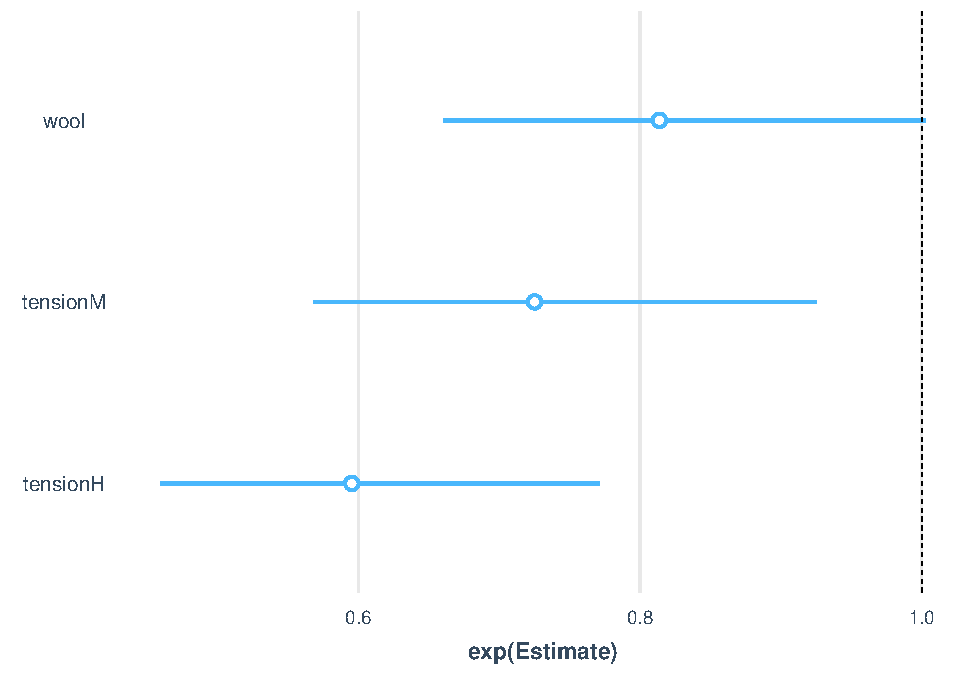
\includegraphics{bookglm_files/figure-latex/unnamed-chunk-39-1.pdf}

\begin{Shaded}
\begin{Highlighting}[]
\CommentTok{\# plot regression coefficients for poisson.model2 and poisson.model}
\FunctionTok{plot\_summs}\NormalTok{(poisson.model, poisson.model2, }\AttributeTok{scale =} \ConstantTok{TRUE}\NormalTok{, }\AttributeTok{exp =} \ConstantTok{TRUE}\NormalTok{)}
\end{Highlighting}
\end{Shaded}

\begin{verbatim}
## Note: Pseudo-R2 for quasibinomial/quasipoisson families is calculated by
## refitting the fitted and null models as binomial/poisson.
\end{verbatim}

\begin{verbatim}
## Loading required namespace: broom.mixed
## Loading required namespace: broom.mixed
\end{verbatim}

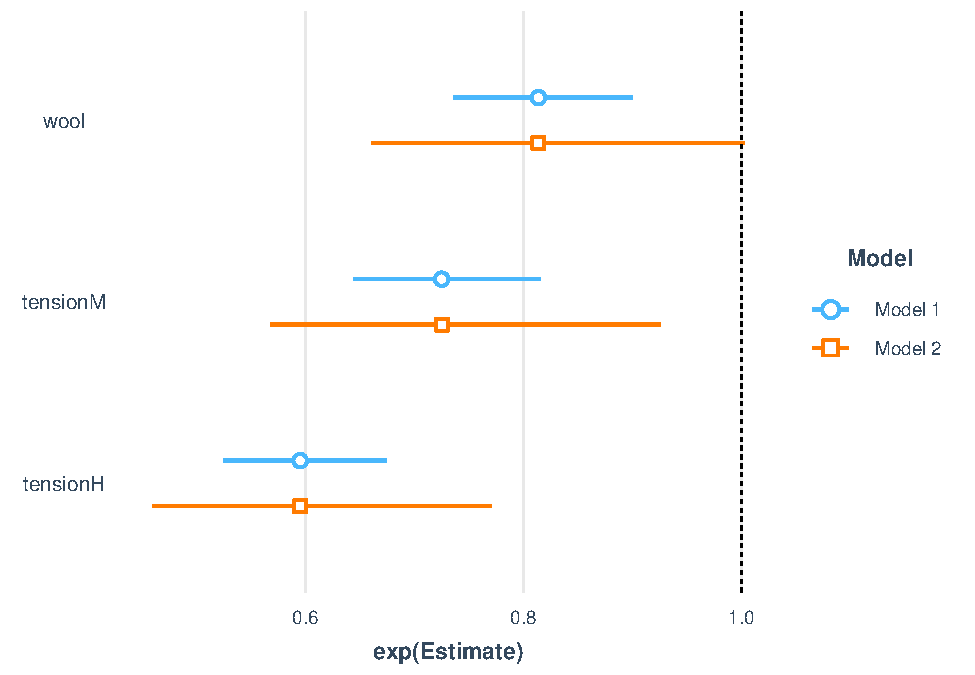
\includegraphics{bookglm_files/figure-latex/unnamed-chunk-40-1.pdf}

En el código anterior, \texttt{plot\_summs\ (poisson.model2,\ scale\ =\ TRUE,\ exp\ =\ TRUE)}traza el segundo modelo usando la familia cuasi-poisson en \texttt{glm}.

El primer argumento en \texttt{plot\_summs\ ()}es el modelo de regresión que se utilizará, puede ser uno o más de uno.

scale ayuda con el problema de las diferentes escalas de las variables.\texttt{exp} se establece en \texttt{TRUE} porque para la regresión de Poisson es más probable que nos interesen los valores exponenciales de las estimaciones en lugar de los lineales.

Puede encontrar más detalles sobre jtools y plot\_summs () aquí en la documentación.

También podemos visualizar la interacción entre variables predictoras.\texttt{jtools} proporciona diferentes funciones para diferentes tipos de variables. Por ejemplo, si todas las variables son categóricas, podríamos usar\texttt{cat\_plot\ ()}para comprender mejor las interacciones entre ellas. Para variables continuas, se usa \texttt{interact\_plot\ ()}.

En los datos de warpbreaks tenemos variables predictoras categóricas, por lo que usaremos \texttt{cat\_plot\ ()}para visualizar la interacción entre ellas, dándole argumentos que especifiquen qué modelo nos gustaría usar, la variable predictora que estamos viendo y la otra variable predictora con la que se combina para producir el resultado.

\begin{Shaded}
\begin{Highlighting}[]
\FunctionTok{library}\NormalTok{(broom)}
\FunctionTok{library}\NormalTok{(jtools)}
\FunctionTok{library}\NormalTok{(ggstance)}
\CommentTok{\#interact\_plot(poisson.model2,pred = wool,modx =tension)}
\CommentTok{\# argument 1: regression model}
\CommentTok{\# pred: The categorical variable that will appear on x{-}axis}
\CommentTok{\# modx: Moderator variable that has an effect in combination to pred on outcome}
\end{Highlighting}
\end{Shaded}

\begin{Shaded}
\begin{Highlighting}[]
\FunctionTok{library}\NormalTok{(jtools)}
\CommentTok{\#install.packages("broom")}
\CommentTok{\#install.packages("ggstance")}
\CommentTok{\#cat\_plot(poisson.model2,pred = wool,modx = tension)}
\CommentTok{\# argument 1: regression model}
\CommentTok{\# pred: The categorical variable that will appear on x{-}axis}
\CommentTok{\# modx: Moderator variable that has an effect in combination to pred on outcom}
\end{Highlighting}
\end{Shaded}

\begin{Shaded}
\begin{Highlighting}[]
\CommentTok{\#cat\_plot(poisson.model2, pred=tension, modx = wool, \#geom = "line")}
\end{Highlighting}
\end{Shaded}

\hypertarget{modelado-de-regresiuxf3n-de-poisson-utilizando-datos-de-tasas}{%
\chapter{Modelado de regresión de Poisson utilizando datos de tasas}\label{modelado-de-regresiuxf3n-de-poisson-utilizando-datos-de-tasas}}

Hasta ahora, en este tutorial, hemos modelado datos de recuento, pero también podemos modelar datos de tasa que predicen el número de recuentos durante un período de tiempo o agrupación. La fórmula para modelar datos de tasa viene dada por: \[\log (\frac{X}{n})=\beta_{0}+\sum \beta_i X_{i}\] esto es equivalente a:

\[\log (X)-\log (n)=\beta_{0}+\sum \beta_{i} X_{i}\]

\[\log (X)=\log (n)+\beta_{0}+\sum \beta_i X_{i}\] Por lo tanto, los datos de tasa se pueden modelar incluyendo el término log(n) con un coeficiente de 1.

Esto se denomina compensación. Este desplazamiento se modela con \texttt{offset()}en R.

Usemos otro conjunto de datos llamado \textbf{eba1977} del paquete \textbf{ISwR} para modelar el modelo de regresión de Poisson para datos de tasas. Primero, instalaremos el paquete:

\begin{Shaded}
\begin{Highlighting}[]
\CommentTok{\# install.packages("ISwR")}
\FunctionTok{library}\NormalTok{(ISwR)}
\end{Highlighting}
\end{Shaded}

Ahora, echemos un vistazo a algunos detalles sobre los datos e imprimamos las primeras diez filas para tener una idea de lo que incluye el conjunto de datos.

\begin{Shaded}
\begin{Highlighting}[]
\FunctionTok{data}\NormalTok{(eba1977)}
\NormalTok{cancer.data }\OtherTok{=}\NormalTok{ eba1977}
\NormalTok{cancer.data[}\DecValTok{1}\SpecialCharTok{:}\DecValTok{10}\NormalTok{, ]}
\end{Highlighting}
\end{Shaded}

\begin{verbatim}
##          city   age  pop cases
## 1  Fredericia 40-54 3059    11
## 2     Horsens 40-54 2879    13
## 3     Kolding 40-54 3142     4
## 4       Vejle 40-54 2520     5
## 5  Fredericia 55-59  800    11
## 6     Horsens 55-59 1083     6
## 7     Kolding 55-59 1050     8
## 8       Vejle 55-59  878     7
## 9  Fredericia 60-64  710    11
## 10    Horsens 60-64  923    15
\end{verbatim}

\begin{Shaded}
\begin{Highlighting}[]
\CommentTok{\# Description}
\CommentTok{\# Lung cancer incidence in four Danish cities 1968{-}1971}
\CommentTok{\# Description:}
\CommentTok{\# This data set contains counts of incident lung cancer cases and}
\CommentTok{\# population size in four neighbouring Danish cities by age group.}
\CommentTok{\# Format:}
\CommentTok{\# A data frame with 24 observations on the following 4 variables:}
\CommentTok{\# city a factor with levels Fredericia, Horsens, Kolding, and Vejle.}
\CommentTok{\# age a factor with levels 40{-}54, 55{-}59, 60{-}64, 65{-}69,70{-}74, and 75+.}
\CommentTok{\# pop a numeric vector, number of inhabitants.}
\CommentTok{\# cases a numeric vector, number of lung cancer cases.}
\end{Highlighting}
\end{Shaded}

Para modelar datos de tasa, usamos \(\dfrac{X}{n}\) donde X es el evento que sucederá y n es la agrupación. En este ejemplo, X = casos (el evento es un caso de cáncer) y n = pop (la población es la agrupación).

Como en la fórmula anterior, los datos de tasa se contabilizan mediante log (n) y en estos datos n es la población, por lo que primero encontraremos el log de la población. Podemos modelar para casos / población de la siguiente manera:

\begin{Shaded}
\begin{Highlighting}[]
\CommentTok{\# find the log(n) of each value in \textquotesingle{}pop\textquotesingle{} column. It is the third column}

\NormalTok{logpop }\OtherTok{=} \FunctionTok{log}\NormalTok{(cancer.data[ ,}\DecValTok{3}\NormalTok{])}

\CommentTok{\# add the log values to the dataframe using \textquotesingle{}cbind()\textquotesingle{}}

\NormalTok{new.cancer.data }\OtherTok{=} \FunctionTok{cbind}\NormalTok{(cancer.data, logpop)}

\CommentTok{\# display new dataframe}
\NormalTok{new.cancer.data}
\end{Highlighting}
\end{Shaded}

\begin{verbatim}
##          city   age  pop cases   logpop
## 1  Fredericia 40-54 3059    11 8.025843
## 2     Horsens 40-54 2879    13 7.965198
## 3     Kolding 40-54 3142     4 8.052615
## 4       Vejle 40-54 2520     5 7.832014
## 5  Fredericia 55-59  800    11 6.684612
## 6     Horsens 55-59 1083     6 6.987490
## 7     Kolding 55-59 1050     8 6.956545
## 8       Vejle 55-59  878     7 6.777647
## 9  Fredericia 60-64  710    11 6.565265
## 10    Horsens 60-64  923    15 6.827629
## 11    Kolding 60-64  895     7 6.796824
## 12      Vejle 60-64  839    10 6.732211
## 13 Fredericia 65-69  581    10 6.364751
## 14    Horsens 65-69  834    10 6.726233
## 15    Kolding 65-69  702    11 6.553933
## 16      Vejle 65-69  631    14 6.447306
## 17 Fredericia 70-74  509    11 6.232448
## 18    Horsens 70-74  634    12 6.452049
## 19    Kolding 70-74  535     9 6.282267
## 20      Vejle 70-74  539     8 6.289716
## 21 Fredericia   75+  605    10 6.405228
## 22    Horsens   75+  782     2 6.661855
## 23    Kolding   75+  659    12 6.490724
## 24      Vejle   75+  619     7 6.428105
\end{verbatim}

Ahora, modelemos los datos de la tasa con \textbf{offset()}

\begin{Shaded}
\begin{Highlighting}[]
\NormalTok{poisson.model.rate}\OtherTok{\textless{}{-}}\FunctionTok{glm}\NormalTok{(cases }\SpecialCharTok{\textasciitilde{}}\NormalTok{ city }\SpecialCharTok{+}\NormalTok{ age}\SpecialCharTok{+} \FunctionTok{offset}\NormalTok{(logpop), }\AttributeTok{family =} \FunctionTok{poisson}\NormalTok{(}\AttributeTok{link =} \StringTok{"log"}\NormalTok{), }\AttributeTok{data =}\NormalTok{ cancer.data)}

\CommentTok{\#display summary}
\FunctionTok{summary}\NormalTok{(poisson.model.rate)}
\end{Highlighting}
\end{Shaded}

\begin{verbatim}
## 
## Call:
## glm(formula = cases ~ city + age + offset(logpop), family = poisson(link = "log"), 
##     data = cancer.data)
## 
## Deviance Residuals: 
##      Min        1Q    Median        3Q       Max  
## -2.63573  -0.67296  -0.03436   0.37258   1.85267  
## 
## Coefficients:
##             Estimate Std. Error z value Pr(>|z|)    
## (Intercept)  -5.6321     0.2003 -28.125  < 2e-16 ***
## cityHorsens  -0.3301     0.1815  -1.818   0.0690 .  
## cityKolding  -0.3715     0.1878  -1.978   0.0479 *  
## cityVejle    -0.2723     0.1879  -1.450   0.1472    
## age55-59      1.1010     0.2483   4.434 9.23e-06 ***
## age60-64      1.5186     0.2316   6.556 5.53e-11 ***
## age65-69      1.7677     0.2294   7.704 1.31e-14 ***
## age70-74      1.8569     0.2353   7.891 3.00e-15 ***
## age75+        1.4197     0.2503   5.672 1.41e-08 ***
## ---
## Signif. codes:  0 '***' 0.001 '**' 0.01 '*' 0.05 '.' 0.1 ' ' 1
## 
## (Dispersion parameter for poisson family taken to be 1)
## 
##     Null deviance: 129.908  on 23  degrees of freedom
## Residual deviance:  23.447  on 15  degrees of freedom
## AIC: 137.84
## 
## Number of Fisher Scoring iterations: 5
\end{verbatim}

En este conjunto de datos, podemos ver que la desviación residual está cerca de los grados de libertad y el parámetro de dispersión es 1.5 (23.447 / 15) que es pequeño, por lo que el modelo es un buen ajuste.

Usamos \texttt{fitted(model)} para devolver valores ajustados por el modelo. Devuelve resultados utilizando los datos de entrenamiento sobre los que se construye el modelo. Hagamos un intento:

\begin{Shaded}
\begin{Highlighting}[]
\FunctionTok{fitted}\NormalTok{(poisson.model.rate)}
\end{Highlighting}
\end{Shaded}

\begin{verbatim}
##         1         2         3         4         5         6         7         8 
## 10.954812  7.411803  7.760169  6.873215  8.615485  8.384458  7.798635  7.201421 
##         9        10        11        12        13        14        15        16 
## 11.609373 10.849479 10.092831 10.448316 12.187276 12.576313 10.155638 10.080773 
##        17        18        19        20        21        22        23        24 
## 11.672630 10.451942  8.461440  9.413988  8.960422  8.326004  6.731286  6.982287
\end{verbatim}

Usando este modelo, podemos predecir el número de casos por 1000 habitantes para un nuevo conjunto de datos, usando la función \texttt{predict\ (),} de manera muy similar a como lo hicimos para nuestro modelo de conteo de datos anteriormente:

\begin{Shaded}
\begin{Highlighting}[]
\CommentTok{\# create a test dataframe containing new values of variables}
\NormalTok{test.data }\OtherTok{=} \FunctionTok{data.frame}\NormalTok{(}\AttributeTok{city =} \StringTok{"Kolding"}\NormalTok{, }\AttributeTok{age =} \StringTok{"40{-}54"}\NormalTok{, }\AttributeTok{pop =} \DecValTok{1000}\NormalTok{, }\AttributeTok{logpop =} \FunctionTok{log}\NormalTok{(}\DecValTok{1000}\NormalTok{))}

\CommentTok{\# predict outcomes (responses) using \textquotesingle{}predict()\textquotesingle{}}
\NormalTok{predicted.value}\OtherTok{\textless{}{-}}\FunctionTok{predict}\NormalTok{(poisson.model.rate, test.data, }\AttributeTok{type =} \StringTok{"response"}\NormalTok{)}

\CommentTok{\# show predicted value}
\NormalTok{predicted.value}
\end{Highlighting}
\end{Shaded}

\begin{verbatim}
##        1 
## 2.469818
\end{verbatim}

Entonces, para la ciudad de Kolding entre las personas en el grupo de edad de 40 a 54 años, podríamos esperar aproximadamente 2 o 3 casos de cáncer de pulmón por cada 1000 personas.

\hypertarget{conclusiuxf3n}{%
\chapter{Conclusión}\label{conclusiuxf3n}}

Los modelos de regresión de Poisson tienen una gran importancia en las predicciones econométricas y del mundo real. En este tutorial, hemos aprendido sobre la distribución de Poisson, los modelos lineales generalizados y los modelos de regresión de Poisson.

También aprendimos cómo implementar modelos de regresión de Poisson para datos de recuento y tasa en R usando glm (), y cómo ajustar los datos al modelo para predecir un nuevo conjunto de datos. Además, analizamos cómo obtener errores estándar más precisos en glm () usando quasipoisson y vimos algunas de las posibilidades disponibles para la visualización con jtools

\hypertarget{variables-binarias-y-regresiuxf3n-loguxedstica.}{%
\chapter{Variables Binarias y regresión Logística.}\label{variables-binarias-y-regresiuxf3n-loguxedstica.}}

\hypertarget{distribuciones-de-probabilidad..}{%
\section{Distribuciones de probabilidad..}\label{distribuciones-de-probabilidad..}}

En este capítulo consideramos modelos lineales generalizados en los que las variables de resultado se miden en una escala binaria. Por ejemplo, las respuestas pueden estar vivas o muertas, presentes o ausentes. El éxito y el fracaso se utilizan como términos genéricos de las dos categorías. Primero, definimos la variable aleatoria binaria
\[
Z = \left\{\begin{array}{l}
1 \quad \text{si el resultado es un éxito} \\
0 \quad \text{si el resultado es un fracaso}
\end{array}\right.
\]
con probabilidades \(\operatorname{Pr}(Z=1) =\pi\) y \(\operatorname{Pr}(Z=0) = 1-\pi\), que es la distribución de Bernoulli \(\mathrm{B}\)(\pi PS Si hay \(n\) tales variables aleatorias \(Z_{1}, \ldots,Z_{n}\), que son independientes con \(\operatorname{Pr}\left(Z_{j} =1\right) = \pi_{j}\), entonces su probabilidad conjunta es
\begin{equation}
\prod_{j=1}^{n} \pi_{j}^{z_{j}}\left(1-\pi_{j} \right)^{1-z_{j}} = \exp\left[\sum_{j=1}^{n}z_{j}\log\left(\frac{\pi_{j}} {1- \pi_{j}} \right) + \sum_{j=1}^{n} \log\left(1-\pi_{j}\right)\right]
\end{equation}
que es un miembro de la familia exponencial.

A continuación, para el caso en el que los \(\pi_{j}\) son todos iguales, podemos definir
\[
Y = \sum_{j=1}^{n}Z_{j}
\]
de modo que \(Y\) es el número de éxitos en \(n\) ``ensayos''. La variable aleatoria \(Y\) tiene la distribución \(\operatorname{Bin}(n, \pi)\)
\begin{equation}
\operatorname{Pr}(Y = y) = \left(\begin{array}{l}
n\\
y
\end{array}\right) \pi^{y}(1- \pi)^{n-y}, \quad y = 0,1, \ldots, n
\end{equation}
Finalmente, consideramos el caso general de \(N\) variables aleatorias independientes
\(Y_{1}, Y_{2}, \ldots, Y_{N}\) correspondientes al número de éxitos en \(N\) diferentes subgrupos o estratos (en la siguiente tabla). Si \(Y_{i}\sim \operatorname{Bin} \left(n_{i}, \pi_{i}\right)\), la función de probabilidad de registro es
\[
\begin{array}{l}
l\left(\pi_{1}, \ldots, \pi_{N} ; y_{1}, \ldots, y_{N}\right) \\
=\sum_{i=1}^{N}\left[y_{i} \log \left(\frac{\pi_{i}}{1-\pi_{i}}\right)+n_{i} \log \left(1-\pi_{i}\right)+\log \left(\begin{array}{l}
n_{i} \\
y_{i}
\end{array}\right]\right.
\end{array}
\]
poner aqui una tabla como imagen dobson

\hypertarget{modelos-lineales-generalizados.}{%
\section{Modelos lineales generalizados.}\label{modelos-lineales-generalizados.}}

Queremos describir la proporción de éxitos, \(P_{i}= \dfrac{Y_{i}}{n_{i}}\), en cada subgrupo en términos de niveles de factores y otras variables explicativas que caracterizan al subgrupo. Como \(\mathrm{E}\left(Y_{i}\right)=n_{i} \pi_{i}\) y así \(\mathrm{E} \left(P_{i}\right)=\pi_{i}\), modelamos las probabilidades \(\pi_{i}\) como
\[
g\left(\pi_{i}\right)=\mathbf{x}_{i}^{T}\boldsymbol{\beta}
\]
donde \(\mathbf{x}_{i}\) es un vector de variables explicativas(variables ficticias para niveles de factor y valores medidos para covariables), \(\boldsymbol{\beta}\) es un vector de parámetros y \(g\) es un función de enlace. El caso más simple es el modelo lineal.
\[
\pi=\mathbf{x}^{T}\boldsymbol{\beta}
\]
Esto se usa en algunas aplicaciones prácticas, pero tiene la desventaja de que aunque \(\pi\) es una probabilidad, los valores ajustados \(\mathbf{x}^ {T}\mathbf{b}\) pueden ser menores que cero o mayores que uno.

Para garantizar que \(\pi\) esté restringido al intervalo \([0,1]\), a menudo se modela utilizando una distribución de probabilidad acumulativa

\[
\pi=\int_{-\infty}^{t}f(s)ds
\]
donde \(f(s)\geqslant 0\) y \(\int_{-\infty}^{\infty}(s)ds=1\). La función de densidad de probabilidad \(f(s)\) se denomina distribución de tolerancia.

\hypertarget{modelos-de-respuesta-a-la-dosis.}{%
\section{Modelos de respuesta a la dosis.}\label{modelos-de-respuesta-a-la-dosis.}}

Históricamente, uno de los primeros usos de modelos de regresión para datos binomiales fue para los resultados de bioensayos (Finney 1973). Las respuestas fueron las proporciones o porcentajes de ``éxitos''; por ejemplo, la proporción de animales de experimentación muertos por distintos niveles de dosis de una sustancia tóxica. A veces, estos datos se denominan respuestas cuánticas. El objetivo es describir la probabilidad de ``éxito'', \(\pi\), en función de la dosis, \(x\); por ejemplo, \(g(\pi) = \beta_{1} + \beta_{2}x\). Si la distribución de tolerancia \(f(s)\) es la distribución uniforme en el intervalo \(\left[c_{1}, c_{2}\right]\)
\[
f (s) = \left\{\begin{array}{cc}
\frac{1}{c_{2} -c_{1}} & \text{if} c_{1} \leqslant s \leqslant c_{2} \\
0 & \text{de lo contrario}
\end{array} \right.
\]
entonces \(\pi\) es acumulativo

\[
\pi = \int_{c_{1}}^{x} f (s) ds = \frac{x-c_ {1}} {c_{2} -c_{1}} \quad \text {para}\quad  c_{1} \leqslant x \leqslant c_{2}
\]
(ver figura \(7.1\)). Esta ecuación tiene la forma \(\pi=\beta_{1} + \beta_{2}x\), donde
\[
\beta_{1} = \frac{-c_{1}} {c_{2} -c_{1}} \quad \text{y} \quad \beta_{2} = \frac{1}{c_{2} -c_{ 1}}
\]

\hypertarget{final-words}{%
\chapter{Final Words}\label{final-words}}

We have finished a nice book.

  \bibliography{book.bib,packages.bib}

\end{document}
